\documentclass[10pt, a4paper,english,spanish]{article}
\usepackage[utf8]{inputenc}
\usepackage[spanish]{babel}
\parindent = 0 pt
\usepackage{geometry}
\usepackage{xr}
\usepackage{placeins}
\usepackage{vmargin}
\setpapersize{A4}
\setmargins{2.5cm}       % margen izquierdo
{1.5cm}                        % margen superior
{16.5cm}                      % anchura del texto
{23.42cm}                    % altura del texto
{2cm}                           % altura de los encabezados
{1cm}                           % espacio entre el texto y los encabezados
{0pt}                             % altura del pie de página
{1cm} 
\usepackage{subfigure}
\usepackage{mathtools}
\DeclarePairedDelimiter\abs{\lvert}{\rvert}
\usepackage{amsmath}
\usepackage{amsfonts}
%\usepackage{amssymb}
%\usepackage[utf8]{inputenc}
\usepackage{graphicx}
%\usepackage{verbatim}
%\usepackage{color}
\usepackage{listings}
\newtheorem{proposition}{Proposici\'on}
\setlength{\parindent}{0.5cm}


\usepackage{color} % para snipets de codigo coloreados
\usepackage{fancybox}  % para el sbox de los snipets de codigo

\definecolor{litegrey}{gray}{0.94}

% \newenvironment{sidebar}{%
% 	\begin{Sbox}\begin{minipage}{.85\textwidth}}%
% 	{\end{minipage}\end{Sbox}%
% 		\begin{center}\setlength{\fboxsep}{6pt}%
% 		\shadowbox{\TheSbox}\end{center}}
% \newenvironment{warning}{%
% 	\begin{Sbox}\begin{minipage}{.85\textwidth}\sffamily\lite\small\RaggedRight}%
% 	{\end{minipage}\end{Sbox}%
% 		\begin{center}\setlength{\fboxsep}{6pt}%
% 		\colorbox{litegrey}{\TheSbox}\end{center}}

\newenvironment{codesnippet}{%
	\begin{Sbox}\begin{minipage}{\textwidth}\sffamily\small}%
	{\end{minipage}\end{Sbox}%
		\begin{center}%
		\colorbox{litegrey}{\TheSbox}\end{center}}



\usepackage{fancyhdr}
\pagestyle{fancy}

%\renewcommand{\chaptermark}[1]{\markboth{#1}{}}
\renewcommand{\sectionmark}[1]{\markright{\thesection\ - #1}}

\fancyhf{}

\fancyhead[LO]{Sección \rightmark} % \thesection\ 
\fancyfoot[LO]{}
\fancyfoot[RO]{\thepage}
\renewcommand{\headrulewidth}{0.5pt}
\renewcommand{\footrulewidth}{0.5pt}
\setlength{\hoffset}{-0.8in}
\setlength{\textwidth}{16cm}
%\setlength{\hoffset}{-1.1cm}
%\setlength{\textwidth}{16cm}
\setlength{\headsep}{0.5cm}
\setlength{\textheight}{25cm}
\setlength{\voffset}{-0.7in}
\setlength{\headwidth}{\textwidth}
\setlength{\headheight}{13.1pt}

\renewcommand{\baselinestretch}{1.1}  % line spacing


% \setcounter{secnumdepth}{2}
\usepackage{caratula}
\usepackage{url}

\begin{document}

\thispagestyle{empty}
\materia{Métodos Numéricos}
\submateria{Segundo Cuatrimestre de 2015}
\titulo{Trabajo Práctico I}
\subtitulo{Discretización de la temperatura de un Alto Horno}
\integrante{Alvarez, Lautaro Leonel}{268/14}{lautarolalvarez@gmail.com}
\integrante{Maddonni, Axel Ezequiel}{200/14}{axel.maddonni@gmail.com}
\integrante{Thibeault, Gabriel Eric}{114/13}{gabriel.eric.thibeault@gmail.com}
\claves{eliminación gaussiana, factorización lu}
\intro{En este trabajo discretizaremos el interior de un alto horno para calcular su temperatura interna e implementaremos un algoritmo para determinar si se encuentra en estado de peligro, usando distintos métodos numéricos para resolver sistemas de ecuaciones lineales planteados a partir de ecuaciones matemáticas que describen dicha situación.}

\maketitle
\newpage

\thispagestyle{empty}
\vfill

\thispagestyle{empty}
\vspace{3cm}
\tableofcontents
\newpage

%\normalsize
\newpage

\section{Introducci\'on Te\'orica}

\subsection{Explicaci\'on de los m\'etodos utilizados}
\subsubsection{Eliminaci\'on Gaussiana}
\par El m\'etodo de Eliminaci\'on Gaussiana se utiliza para triangular superiormente una matriz. Esto se logra iterando sobre filas, utilizando un pivote diagonal (que llamaremos $i$ en la siguiente explicaci\'on por claridad); en cada iteraci\'on del ciclo exterior se resta a cada una de las filas inferiores a la i-\'esima, la i-\'esima multiplicada por un coeficiente tal que el elemento de la i-\'esima columna quede en 0. Al iterar sobre todas las filas (excepto la \'ultima, ya que no tiene filas inferiores a ella), se triangula la matriz. Al restarle una fila a otra, tambi\'en se restan los t\'erminos independientes correspondientes a cada fila de la misma forma.
\par Una optimizaci\'on que incorporamos es no restar las filas si el elemento a dejar en 0 ya est\'a en 0. Como la matriz que representa el problema es Banda (esta proposici\'on se encuentra demostrada en la secci\'on \ref{subsec:DemBanda}), y por ende deber\'ia tener una significante cantidad de valores en 0, esta optimizaci\'on deber\'ia ser considerablemente efectiva.
\subsubsection{Descomposici\'on LU}
\par La Descomposici\'on LU es similar a la Eliminaci\'on Gaussiana, pero al restarle la fila i-\'esima multiplicada por el coeficiente ($i$ siendo el pivote diagonal detallado en la secci\'on anterior) a la j-\'esima ($j$ siendo el \'indice de la fila sobre la cual se itera en el ciclo interno), se guarda tal coeficiente como el $j,i$-\'esimo valor de una nueva matriz. Los valores de la diagonal de la nueva matriz se inicializan en 1, y el resto en 0, y por la forma en que se itera para triangular superiormente una matriz, \'esta queda triangular inferior. 
\par La diferencia principal de la Descomposici\'on LU respecto de la Eliminaci\'on Gaussiana es que no involucra al t\'ermino independiente, y una vez descompuesta una matriz, se puede resolver el sistema para cualquier t\'ermino independiente. Ya que la complejidad de resolver un sistema triangular (o dos, en el caso de LU) es $O(n^2)$ ($n$ siendo el tama\~no de la matriz), y el de la Descomposici\'on LU o Gauss es $O(n^3)$, si se debe resolver el mismo sistema con distintos t\'erminos independientes, LU deber\'ia ser el m\'etodo superior, ya que s\'olo se debe pagar una vez el coste c\'ubico.
\par Utilizamos la misma optimizaci\'on para matriz banda con LU que mencionamos en la secci\'on anterior.
\subsubsection{Resolver un sistema triangular}
\par Para resolver un sistema triangular se itera por filas (comenzando a partir de la fila con un \'unico valor no-nulo), y se despeja el valor de la diagonal, rest\'andole al t\'ermino independiente todos los otros coeficientes por el valor de sus variables (que, si se itera correctamente, ya deber\'ian haber sido calculadas). Resolver un sistema triangular inferior es similar a resolver un sistema triangular superior, pero se comienza a iterar en distintos puntos y se deben despejar los valores de distintos lados de la diagonal (ya que los sistemas son triangulares no hace falta despejar todos los valores de la fila, ya que se sabe de antemano que los de un lado son todos 0).
\subsubsection{Resolver un sistema LU}
\par Resolver un sistema que fue descompuesto mediante LU consiste en encontrar la soluci\'on de la matriz triangular inferior con el t\'ermino independiente original, y luego la matriz triangular superior utilizando como t\'ermino independiente a la soluci\'on reci\'en encontrada para la matriz inferior.

 
\newpage
 
\section{Desarrollo}

\subsection{Presentaci\'on del problema y explicaci\'on del m\'etodo de discretizaci\'on}
Para averiguar la posici\'on de la isoterma debemos determinar la temperatura en cada punto de la pared. Al sernos imposible resolver el problema computacionalmente decidimos discretizar el problema, por lo que vamos a buscar las temperaturas cada una cierta distancia (la cual variaremos para experimentar los cambios en los resultados). Identificaremos as\'i un punto de la pared por su distancia al centro del horno (r) y su \'angulo ($\theta$) con respecto a un eje fijo.

Para determinar la temperatura en un punto contamos con la siguiente ecuaci\'on:

\begin{equation}\label{calor}
\frac{\partial^2T(r,\theta)}{\partial r^2}+\frac{1}{r}\frac{\partial T(r,\theta)}{\partial r}+\frac{1}{r^2}\frac{\partial^2T(r,\theta)}{\partial \theta^2} = 0 
\end{equation}

Siendo T($r$,$\theta$) la funci\'on que nos da como resultado la temperatura en un punto de radio r y \'angulo $\theta$.

Discretizamos tomando r$_i$ = r$_0$ \textless r$_1$ \textless ... \textless r$_n$ = r$_e$ (con r$_i$=radio interno y r$_e$=radio externo) y 0 = $\theta _0$ \textless $\theta _1$ \textless ... \textless $\theta _m$ = 2$\pi$, tomando así n+1 radios y m \'angulos. Por ende tomamos un t que cumple: t$_{i,j}$ = T(r$_i$,$\theta _j$) (temperatura en el punto con distancia r$_i$ al centro y \'angulo $\theta _j$).

Por ende tomamos la ecuaci\'on \ref{calor} y discretizando tenemos:

\begin{equation}
\label{EcuacionLaPlace}
\frac{t_{i-1,j}-2t_{i,j}+t_{i+1,j}}{(\Delta r)^2}+\frac{1}{r}\frac{t_{i+1,j}-t_{i,j}}{\Delta r}+\frac{1}{r^2}\frac{t_{i,j-1}-2t_{i,j}+t_{i,j+1}}{(\Delta \theta)^2}
\end{equation}

Con $\Delta r$ = r$_i$ - r$_{i-1}$ para i=1..n y $\Delta \theta$ = $\theta _j$ - $\theta _{j-1}$ para j=1..m.

Como vemos en la ecuaci\'on \ref{EcuacionLaPlace} la temperatura en un punto i,j (t$_{i,j}$) depende de las temperatura de los 4 puntos mas cercanos (t$_{i-1,j}$, t$_{i+1,j}$, t$_{i,j-1}$, t$_{i,j+1}$).

Si planteamos un sistema de ecuaciones con 1 ecuaci\'on para cada i,j de la discretizaci\'on obtenemos un sistema de n*m ecuaciones donde cada una depende de 5 temperaturas. Al mismo tiempo sabemos de antemano los valores de los puntos externos e internos, teniendo en cuenta que tomamos como par\'ametros conocidos la temperatura en el borde externo de la pared (T$_e$) y la temperatura en el borde interno de la pared (T$_i$).

\begin{figure}[ht]
\begin{center}
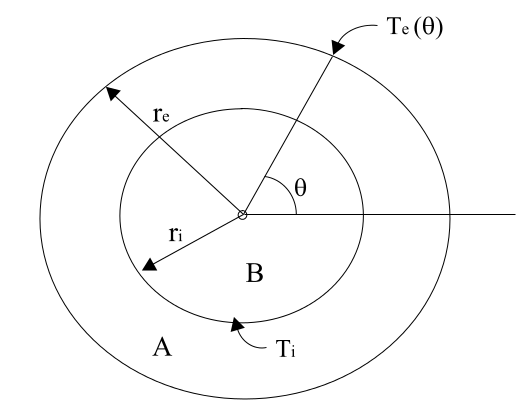
\includegraphics[width=0.4\columnwidth]{../tp1-package/docs/Horno.png}
\end{center}
\end{figure}

De esta forma, podemos plantear una matriz que cumple con la propiedad de ser banda, y con la cual además, es posible realizar Eliminación Gaussiana sin pivoteo (esta propiedad está demostrada más adelante).

\subsection{Armado de la Matriz Banda}
\label{subsec:DemBanda}

\par Para generar la matriz es necesario realizar una transformaci\'on del espacio polar en el que existen los puntos del horno (cuyas posiciones est\'an dadas por \'angulo y radio) a un vector de dimensi\'on (m + 1) * n (este valor corresponde con la cantidad de puntos en la discretizacio\'n). 
\par La transformaci\'on utilizada es bastante simple: 
\begin{equation}
f(j, k)\ =\ j * n + k
\label{eqTransf}
\end{equation}
donde f es la transformaci\'on, j representa que el elemento es el j-\'esimo en la componente del radio, k el equivalente para el \'angulo, y n es la cantidad de puntos de la discretizaci\'on con igual radio (la cantidad de puntos en cada c\'irculo conc\'entrico del horno).
\par De acuerdo a la ecuaci\'on \ref{EcuacionLaPlace}, para cada punto $p_{j, k}$ (cuya ecuaci\'on se encuentra representada en la fila $f(j, k)$) que no pertenece ni al radio externo ni al interno, los \'unicos coeficientes no-nulos en su fila corresponden a los puntos $p_{j-1, k}$, $p_{j+1, k}$, $p_{j, k}$, $p_{j, k-1}$, $p_{j, k+1}$; siendo los sub\'indices la posici\'on de cada punto en la discretizaci\'on. 
Utilizando la ecuaci\'on \ref{eqTransf}, estas posiciones corresponden a las siguientes columnas, respectivamente: $(j-1) * n + k$, $(j+1) * n + k$, $j * n + k$, $j * n + k - 1$, $j * n + k + 1$. 
\par k, como se ha dicho, representa al k-\'esimo elemento con radio j; ya que hay n elementos con igual radio, $0\leq k\leq n$. Por ende, para $j > 0$ ($j = 0$ corresponde al radio interno, por lo que este caso no nos concerniene en este momento), $j * n >= k$. 
Por lo tanto, la posici\'on de los valores de la diagonal en cada fila es $j*n+k$, y los valores no-nulos m\'as alejados corresponden a $(j-1) * n + k$ y $(j+1) * n + k$, que entonces equidistan $n$ de la diagonal. 
\par Es decir, se cumple la propiedad de banda para todas las filas de la matriz que no pertenecen al radio interno o externo, y el ancho de la banda es $n+1$. 
Sin embargo, queda justificar que la propiedad de banda se cumple para todas las dem\'as filas. 
Esto es simple de probar, ya que los valores de temperatura de cada uno de los puntos de estos radios son conocidos, y su ecuaci\'on est\'a simplemente dada por $t_{j, k}\ =\ b_{j, k}$; donde el primer t\'ermino representa la temperatura del punto y el segundo el valor del t\'ermino independiente determinado por la entrada.
Por lo tanto, el \'unico coeficiente no-nulo de las filas de los radios externo e interno son los de la diagonal, cuyo valor es 1.
Ya que todos los otros valores son nulos, en particular lo son los que distan m\'as que $n$ de la diagonal, y por ende la matriz es banda. Adicionalmente, hay $n$ puntos en el radio interno, por lo que la altura de la banda tambi\'en es $n+1$.
\par El algoritmo que crea la matriz en cuestión se encuentra en el apéndice B con comentarios incluidos, junto con el algoritmo correspondiente al método de Eliminación Gaussiana con aprovechamiento de matriz banda.

%\begin{figure}[ht]
%\begin{center}
%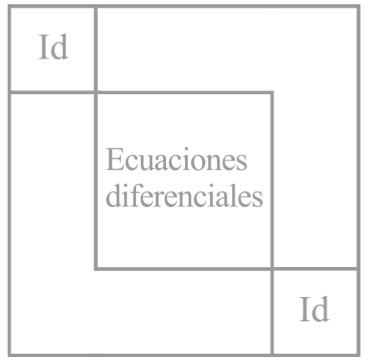
\includegraphics[width=0.4\columnwidth]{imagenes/banda.png}
%\caption{Armado de la Matriz Banda}
%\end{center}
%\end{figure}


\subsection{Demostración: Eliminación Gaussiana sin pivoteo}

\textbf{Proposici\'on}
\hfill{}
Sea $A \in \mathbb{R}^{n \times n}$ la matriz obtenida para el sistema. Es posible aplicar Eliminaci\'on Gaussiana sin pivoteo.

\subsubsection{Lema}

\par Sea $A \in \mathbb{R}^{n \times n}$ la matriz obtenida para el sistema, banda con ancho y alto $n+1$ (como se demostr\'o previamente). 
La \'ultima diagonal superior que pertenece a la banda, tiene (para los valores correspondientes a los radios no-externo y no-internos) coeficientes positivos.
Adicionalmente, al aplicar Eliminaci\'on Gaussiana estos coeficientes nunca se modifican. \newline

\textbf{}
\textbf{}
\textbf{Demostraci\'on del Lema}

\par El hecho que los coeficientes iniciales de la \'ultima diagonal (superior) de la banda sean positivos se desprende de las ecuaciones de cada punto, y ya se explic\'o previamente.
El hecho de que \'estos no se modifiquen al aplicar Gauss se debe a la estructura banda de la matriz:
\begin{equation}
A_{i, j} = 0\ si\ j < i - (n+1) \vee j > i + (n +1)
\end{equation}
\par Entonces, si $j = i + (n+1)$ (como es el caso de la \'ultima diagonal superior de la banda), para una fila $i$, para todas las filas anteriores $k < i$, $j > k + (n+1)$, por lo que $A_{k, j} = 0$.
Al ser $0$, al aplicar Gauss no se alterar\'a el valor del coeficiente.

\subsubsection{Demostraci\'on de la proposici\'on}

\par Ya detallamos que la ecuaci\'on de cada punto indica que en cada fila, la diagonal m\'as la suma de todos los otros coeficientes (no nulos, y luego de todos) es 0. Es decir:
\begin{equation}
A_{i, i} = - (\sum_{j\neq i} A_{i, j})
\end{equation}
\par Por ende, 
\begin{equation}
    \abs{A_{i, i}} = \abs{(\sum_{j\neq i} A_{i, j})} = (\sum_{j\neq i} \abs{A_{i, j}}) \geq (\sum_{j\neq i} \abs{A_{i, j}})
\end{equation}
\par El m\'odulo de la suma es igual a la suma de los m\'odulos ya que todos los coeficientes son no-negativos.
De acuerdo a la ecuaci\'on anterior, la matriz es diagonal dominante (aunque no estrictamente).
\par Demostraremos por inducci\'on que dadas estas propiedades, se puede realizar Eliminaci\'on Gaussiana sin pivoteo.\newline
\newline
\textbf{Caso Base}


\par El caso base consiste en la matriz creada inicialmente, que como ya se demostr\'o, es diagonal dominante, y los valores de su diagonal son no-nulos (para los radios interno y externo valen 1, y
para los otros ya se demostr\'o que son no-nulos).\newline
\newline
\textbf{}
\textbf{Paso Inductivo}


\par Si A tras realizar $k$ iteraciones de Gauss sin pivotaje es diagonal dominante, con $A_{k, k}$ (es decir, el $k$-\'esimo valor de la diagonal) no-nulo, entonces A tras realizar $k+1$ iteraciones de Gauss sin pivotaje es diagonal dominante, con $A_{k+1, k+1}$ no-nulo.
\par Demostraremos primero que A tras realizar $k+1$ iteraciones es diagonal dominante.
Restamos cada fila inferior a la $k$ por el coeficiente correcto:
\begin{equation}
A_j - (A_{j, k} / A_{k, k}) * A_k
\end{equation}
\par Sabemos que es posible hacer esto ya que por Hip\'otesis Inductiva $A_{k, k} \neq 0$.
Sea
\begin{equation}
A_{i, j}^{(2)} = A_{i, j} - (A_{i, k} / A_{k, k}) * A_{k, j}
\end{equation}
\par Quiero ver que:
\begin{equation}
\sum_{j\neq\ i}\abs{A_{i, j}^{(2)}}\leq\ \abs{A_{i, i}^{(2)}}
\end{equation}
\par Veamos que esto sucede:
\begin{equation}
\sum_{j\neq\ i}\abs{A_{i, j} - (A_{i, k} / A_{k, k}) * A_{k, j}}
\end{equation}
\par Por Desigualdad Triangular:
\begin{equation}
    ...\ \leq\ \sum_{j\neq\ i}\abs{A_{i,j}} + \sum_{j\neq\ i}\abs{(A_{i, k} / A_{k, k})}
\end{equation}
\par Por Hip\'otesis Inductiva:
\begin{equation}
    ...\ \leq\ \abs{A_{i, i}} - \abs{A_{i, k}} + (\abs{A_{i, k}}/ \abs{A_{k, k}})*(\sum_{j\neq i}\abs{A_{k, j}})
\end{equation}
\begin{equation}
    ...\ \leq\ \abs{A_{i, i}} - \abs{A_{i, k}} + (\abs{A_{i, k}}/ \abs{A_{k, k}})*(\abs{A_{k, k}}-\abs{A_{k, i}})
\end{equation}
\begin{equation}
    ...\ \leq\ \abs{A_{i, i}} - \abs{A_{i, k}} * \abs{A_{k, i}} / \abs{A_{k, k}}
\end{equation}
\begin{equation}
    ...\ \leq\ \abs{A_{i, i}} 
\end{equation}
\par Finalmente, llegamos a que cada fila donde se rest\'o por Gauss sin pivotaje mantiene su propiedad de diagonalidad dominante (no estricta).
\par Probamos la primera de las dos propiedades que quer\'iamos demostrar: a\'un queda justificar que $A_{k+1, k+1}$ es no-nulo luego de la $k+1$-\'esima iteraci\'on.
+Afortunadamente, esta demostraci\'on es m\'as simple. Utilizando la misma notaci\'on que en la demostraci\'on de la propiedad anterior:
\begin{equation}
A_{k+1, k+1}^{(2)} = A_{k+1, k+1} - (A_{k+1, k} / A_{k, k}) * A_{k, k+1}
\end{equation}
\par En particular, queremos ver que $A_{k+1, k+1}^{(2)}\neq\ 0$:
\begin{equation}
A_{k+1, k+1}^{(2)} \neq 0\ \iff A_{k+1, k+1} - (A_{k+1, k} / A_{k, k}) * A_{k, k+1} \neq 0
\end{equation}
\par De esto se desprende:
\begin{equation}
A_{k+1, k+1} \neq (A_{k+1, k} / A_{k, k}) * A_{k, k+1}
\end{equation}
\par Aplicando m\'odulo de ambos lados de la inecuaci\'on:
\begin{equation}
    \abs{A_{k+1, k+1}} \neq \abs{(A_{k+1, k}} / \abs{A_{k, k})} * \abs{A_{k, k+1}}
\end{equation}
\par Por Hip\'otesis Inductiva, sabemos que 
\begin{equation}
    \abs{A_{k+1, k+1}} \geq \abs{(A_{k+1, k}} 
\end{equation}
\begin{equation}
    \abs{A_{k, k})} \geq \abs{A_{k, k+1}}
\end{equation}
\par La \'unica forma en que se podr\'ia anular $A_{k+1, k+1}$ es si ambos valores de la diagonal son exactamente iguales a $A_{k, k+1}$ y $A_{k+1, k}$, respectivamente.
\par Sin embargo, esto no puede suceder, debido al Lema que demostramos al comienzo de esta prueba: los valores de la \'ultima diagonal de la banda (que debido a la forma de la matriz, nunca ser\'an
$A_{k, k+1}$ o $A_{k+1, k}$) son no-nulos (y en particular positivos, pero con no-nulos alcanza). Si pasara que $\abs{A_{k, k})} = \abs{A_{k, k+1}}$ (o lo mismo para el otro par de valores), entonces:
\begin{equation}
    \abs{A_{k, k})} < \abs{A_{k, k+1}} + \abs{A_{k, k+(n+1)}}
Add a comment to this line
\end{equation}
\par Esto es absurdo, ya que por Hip\'otesis Inductiva, A es diagonal dominante.
\par $QED$.



\subsection{Planteo de Algoritmos}
\par Para el armado de los algoritmos partimos de una división de los subproblemas a resolver:
\begin{itemize}
\item Crear la matriz en base al archivo de entrada, calculando los coeficientes a partir de las ecuaciones y ordenándolos de tal forma que quede banda, como se explicó anteriorimente.
\item Resolver la matriz con el método de Gauss.
\item Calcular la L y la U.
\item Resolver en base a una L y una U.
\item Calcular la isoterma, con dos métodos diferentes: el primero, calculando el radio más cercano al valor buscado por cada ángulo; y el segundo, aproximando un valor entre los dos radios más cercanos al valor buscado.
\item Determinar si es peligroso, de dos maneras diferentes: la primera viendo si algún punto de la isoterma sobrepasa un radio predeterminado cercano al radio externo, y la segunda calculando el porcentaje de puntos que sobrepasan dicho límite. 
\end{itemize}

\par Algunos algoritmos los planteamos basándonos en sus versiones conocidas (y vistas en clase): método de Gauss y calculo de la L y la U. Luego los modificamos de acuerdo a algunos temas de optimización y detalles para las entradas particulares del problema a resolver.
\par Pasamos por una etapa de prueba de los algoritmos, tanto individualmente como en conjunto, donde tuvimos que dedicarnos a algunos errores que surgieron en cuanto a índices y casos borde.
\par Una vez terminados, optimizamos el algoritmo de Eliminación Gaussiana para matrices Banda. Como se puede ver en el apéndice B, el código aprovecha la propiedad de los 0s fuera de la sección diagonal para realizar menos iteraciones.
\par Teníamos planteado implementar las estructuras para aprovechar la propiedad de banda y reducir la complejidad espacial del algoritmo, pero por cuestiones de tiempo, decidimos enfocarnos en la experimentación y discusión.
\par Finalmente nos dedicamos a aproximar la isoterma de mejor manera y pasamos a experimentar. 

\subsection{Planteo de Mediciones Experimentales}

\par Dividiremos los experimentos realizados en tres secciones, dependiendo el aspecto del algoritmo que se quiere medir y comparar.
\begin{itemize}


\item Complejidad Temporal: experimentos que apuntan a comparar el costo en tiempo de ejecución de los algoritmos, dependiendo del nivel de la granularidad (Experimento 1), del método escogido con temperaturas dinámicas, Gauss o LU (Experimento 2), y la comparación con el método que aprovecha el hecho de que la matriz sea banda (Experimento 3).
\item Isoterma: experimentos que apuntan a comparar cómo varía la isoterma devuelta por el algoritmo modificando la granularidad de los radios (Experimento 4), granularidad de los ángulos (Experimento 5) y granularidad de radios y ángulos a la vez (Experimento 6). Además, se comparan dos métodos para calcular la isoterma: el primero, redondeando el resultado al radio más cercano correspondiente al valor buscado en cada ángulo; y el segundo, que calcula un promedio entre los radios más cercanos al valor buscado (Experimento 7). Un último experimento (Experimento 8) busca corroborar si vale la pena aumentar la granularidad para obtener resultados más precisos, en contraposición con un método menos costoso pero de menor precisión.
\item Peligrosidad: experimentos que buscan comparar los dos métodos implementados para calcular la peligrosidad del horno según la isoterma (Experimento 9). El primer método, más brusco, busca solamente si un punto de la isoterma haya traspado el valor de la isoterma 500, mientras que el segundo, realiza un cálculo de porcentaje para calcular si la cantidad de puntos del horno en peligro supera un umbral predeterminado.
\end{itemize}


 
\newpage
 
\section{Resultados y Discusi\'on}

\subsection{Resultados con respecto al Tiempo de ejecuci\'on}

\subsubsection{Experimento 1}
\par El primer experimento consiste en correr el programa, variando la granularidad (en particular la del par\'ametro $m+1$, que determina la cantidad de puntos para cada \'angulo), con $ninst = 1$.
Se busca comparar el tiempo de ejecuci\'on de los distintos algoritmos para resolver un s\'olo sistema, con un \'unico t\'ermino independiente (a esto se debe $ninst = 1$).
Se espera que la Eliminaci\'on Gaussiana optimizada para banda se ejecute m\'as r\'apido que las otras, y que la Descomposici\'on LU sea la m\'as lenta, ya que se deben resolver dos sistemas en vez de uno s\'olo en el caso de Gauss.
El experimento consiste en correr 25 veces cada algoritmo con una serie de entradas en las cuales se mantienen constantes todos los par\'ametros excepto $m+1$ (es decir, variando s\'olo la granularidad). 
\par Se mide el tiempo que tardan en correr estas 25 iteraciones para cada entrada y m\'etodo de resoluci\'on del sistema lineal.
Se utiliza este m\'etodo de medici\'on en vez del promedio ya que ambos son similares (dan los mismos resultados, pero divididos o no por el tama\~no de la muestra), pero debido a la precisi\'on de la herramienta utiliza ($time$ de bash) preferimos dar el tiempo total para perder la menor precisi\'on posible.
\FloatBarrier

\subsubsection{Resultados del Experimento 1} 
\begin{figure}[ht]
\begin{center}
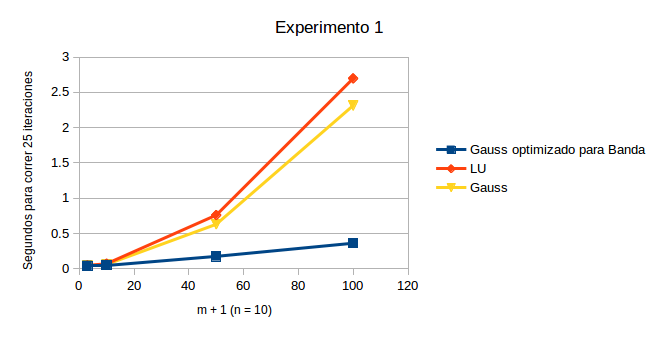
\includegraphics[width=0.8\columnwidth]{../src/experimentos/exp1-3/exp1figura}
\caption{Tiempo de ejecuci\'on en funci\'on del tama\~no de entrada, para ninst = 1}
\label{fig:figura1}
\end{center}
\end{figure}

\par Los resultados del experimento 1 se pueden observar en la figura \ref{fig:figura1}. \'Estos son los esperados: la Eliminaci\'on Gaussiana optimizada es la implementaci\'on m\'as r\'apida, seguida por la Eliminaci\'on Gaussiana (no optimizada), y la Descomposici\'on LU siendo la m\'as lenta.
Cabe destacar la forma cuadr\'atica de la curva del algoritmo de Gauss optimizado, comparada con la forma c\'ubica de las otras dos curvas. 
Ya que $n$ se mantiene constante, el ancho de la banda (que, como se mencion\'o previamente es $n+1$) tambi\'en se mantiene constante, y por ende la complejidad del algoritmo se vuelve $O(tamano de la matriz^2)$, en vez de $O(tamano de la matriz^3)$, y el resultado obtenido es lo esperado.

\FloatBarrier

\subsubsection{Experimento 2}

\par El segundo experimento consiste en correr el programa, con un mismo tama\~no de entrada, pero variando $ninst$. 
El prop\'osito de este experimento es observar como var\'ia el tiempo de ejecuci\'on de los distintos algoritmos para sistemas con varios t\'erminos independientes.
\par Se espera que LU sea m\'as r\'apido que Gauss, ya que s\'olo debe descomponer una vez al sistema y luego puede obtener la soluci\'on para distintos t\'erminos independientes solamente resolviendo
dos sistemas triangulares (que se hace en tiempo $O(tamano de la matriz^2)$. 
\par Sin embargo, la relaci\'on entre el tiempo de ejecuci\'on del algoritmo LU (que tiene un costo inicial de $O(tamano de la matriz^3)$, pero que al aumentar $ninst$, deber\'ia ser opacado por los costos de resolver m\'ultiples veces el sistema en $O(tamano de la matriz^2)$) y Gauss optimizado para Banda (que resuelve una sola vez el sistema, pero debe triangularlo cada vez en $O(tamano de la matriz^2)$) no es conocida de antemano; este tiempo es igual desde el punto de vista de la notaci\'on $O$ grande, pero las constantes escondidas resultar\'an en uno de los m\'etodos sobrepasando al otro.
\FloatBarrier

\subsubsection{Resultados del Experimento 2}


\begin{figure}[ht]
\begin{center}
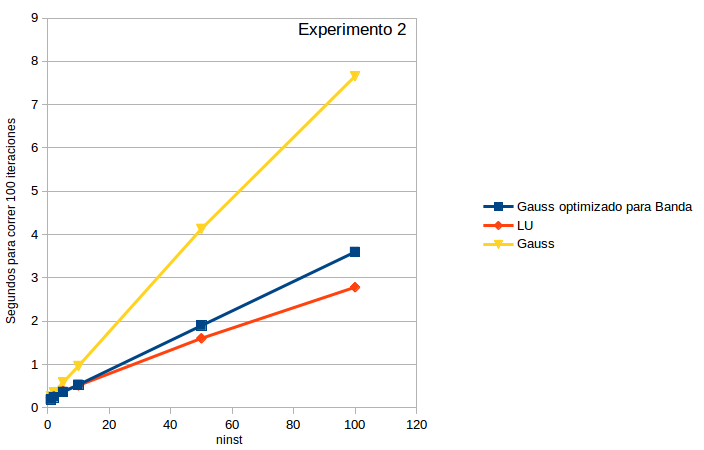
\includegraphics[width=0.8\columnwidth]{../src/experimentos/exp1-3/exp2figuratodos}
\caption{Tiempo de ejecuci\'on en funci\'on de ninst. Gr\'afico con todos los resultados del experimento.}
\label{fig:figura2}
\end{center}
\end{figure}

\begin{figure}[ht]
\begin{center}
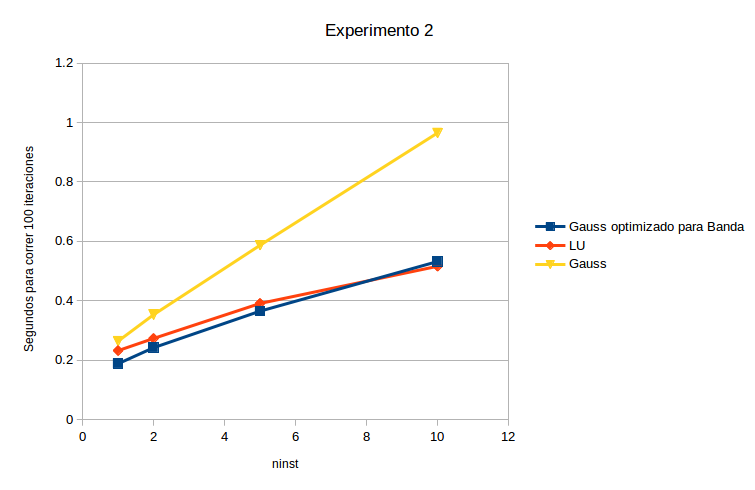
\includegraphics[width=0.8\columnwidth]{../src/experimentos/exp1-3/exp2figurahasta10}
\caption{Tiempo de ejecuci\'on en funci\'on de ninst. Gr\'afico con los valores hasta ninst = 10}
\label{fig:figura3}
\end{center}
\end{figure}


\par Los resultados del experimento 2 se pueden observar en las figuras \ref{fig:figura2} y \ref{fig:figura3} (esta \'ultima representa los mismos resultados que la anterior, pero s\'olo para $ninst\leq10$, para mayor claridad).
Si bien los resultados concernientes a la Eliminaci\'on Gaussiana son los esperados, la relaci\'on entre el tiempo de ejecuci\'on de LU y Gauss optimizado es interesante: para valores peque\~nos de $ninst$, Gauss optimizado es m\'as r\'apido, pero para valores grandes LU lo es.
Esto se debe a que resolver los sistemas de LU tiene un costo menor que triangular y resolver los sistemas utilizando Gauss optimizado; sin embargo, para valores peque\~nos de $ninst$, el costo c\'ubico de la Descomposici\'on LU tiene un mayor peso.

\FloatBarrier

\subsubsection{Experimento 3}
\par El experimento 3 consiste en correr los algoritmos, variando $m+1$ y $n$, pero manteniendo $(m+1)*n$ constante.
El prop\'osito de este experimento es observar como var\'ia el tiempo de ejecuci\'on de los algoritmos al variar s\'olo el ancho y el alto de la banda (que, como se demostr\'o previamente, equivalen a $n+1$), pero manteniendo constante la dimensi\'on de la matriz.
Se espera ver una clara diferencia en lo concerniente al algoritmo optimizado para banda. Los algoritmos de Gauss y LU, tienen una menor optimizaci\'on para banda (que fue detallada en la Introducci\'on Te\'orica), pero no se sabe de antemano cu\'an efectiva es.

\FloatBarrier

\subsubsection{Resultados del Experimento 3}

\begin{figure}[ht]
\begin{center}
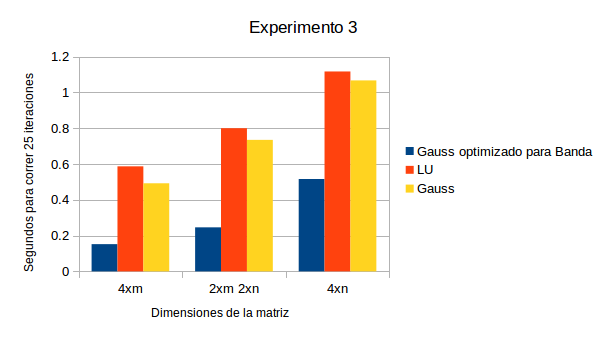
\includegraphics[width=0.8\columnwidth]{../src/experimentos/exp1-3/exp3figura}
\caption{Tiempo de ejecuci\'on para banda de distinto tama\~no, con dimensi\'on de la matriz constante.}
\label{fig:figura4}
\end{center}
\end{figure}

\par Los resultados del experimento 3 se pueden observar en la figura \ref{fig:figura4}. Como era de esperar, se incrementa el tiempo de ejecuci\'on del algoritmo de Gauss optimizado para banda al incrementar el ancho y alto de \'esta; sin embargo, es interesante notar que tambi\'en se incrementa el tiempo de ejecuci\'on de los otros dos algoritmos, y de forma considerable, lo que nos demuestra que la optimizaci\'on mencionada tiene un efecto significante sobre la velocidad de los m\'etodos.
\FloatBarrier

\subsection{Resultados con respecto a la Isoterma}

\subsubsection{Experimento 4}
\par En este experimento se busca comparar los resultados obtenidos en las temperaturas del horno y en el cálculo de la isoterma variando la granularidad de los radios. Para ello tomaremos dos inputs de entrada con los mismos valores de temperatura interna y externa (1500 y 0 respectivamente), mismos radio interno e externo (10 y 100) y misma cantidad de ángulos (30). El primero (4a) dividirá el horno en 10 radios, mientras que el segundo (4b) lo hará en 100. Conjeturamos que al tener más granularidad con respecto a los radios, se obtendrá una isoterma con menos imperfecciones, permitiendo evaluar la peligrosidad de manera más precisa.
\FloatBarrier

\subsubsection{Resultados del experimento 4}

\begin{figure}[ht]
\begin{center}
\subfigure [4a - 10 radios] {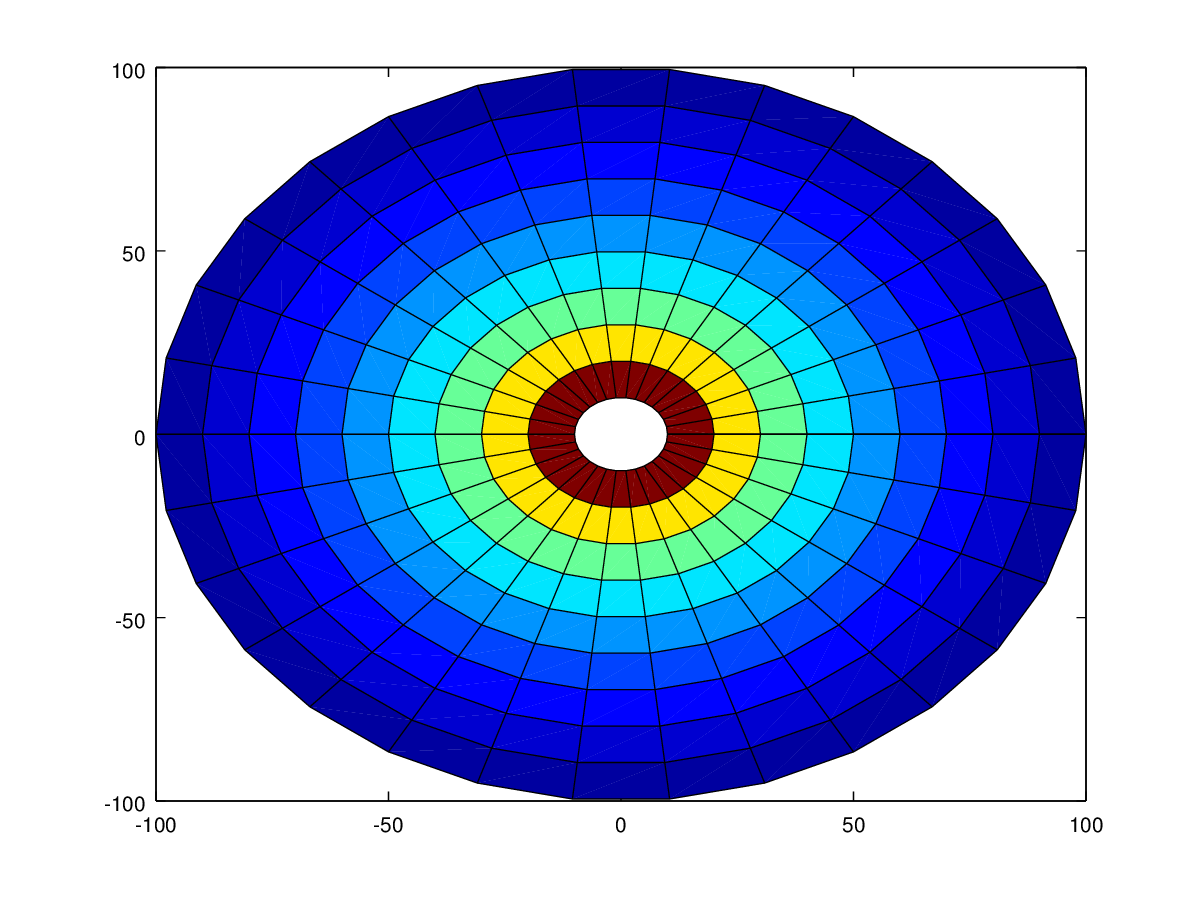
\includegraphics[width=0.49\columnwidth]{../src/experimentos/exp4/calor4A.png}}
\subfigure [4b - 100 radios] {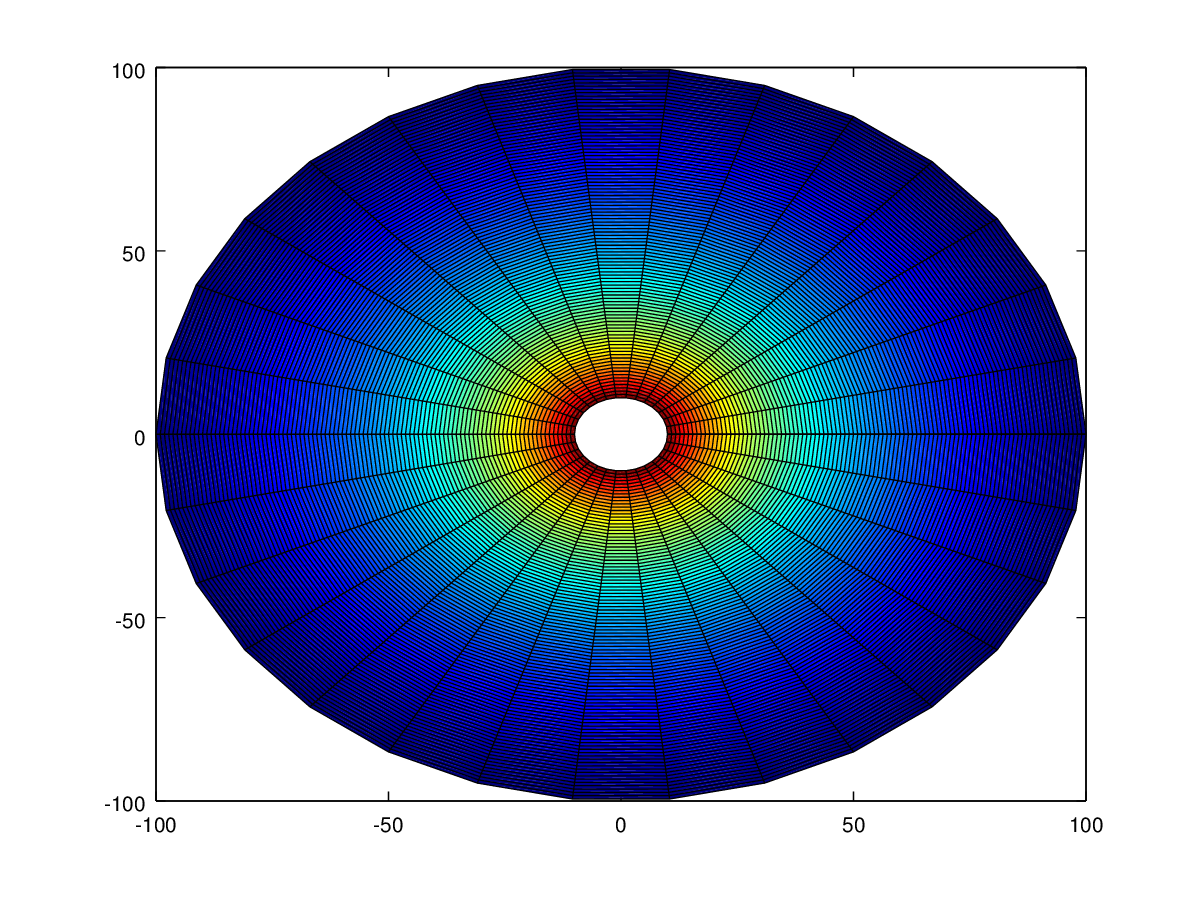
\includegraphics[width=0.49\columnwidth]{../src/experimentos/exp4/calor4b.png}}
\caption{Experimento 4, gráfico de calor}
\end{center}
\end{figure}

\begin{figure}[ht]
\begin{center}
\subfigure [4a - 10 radios] {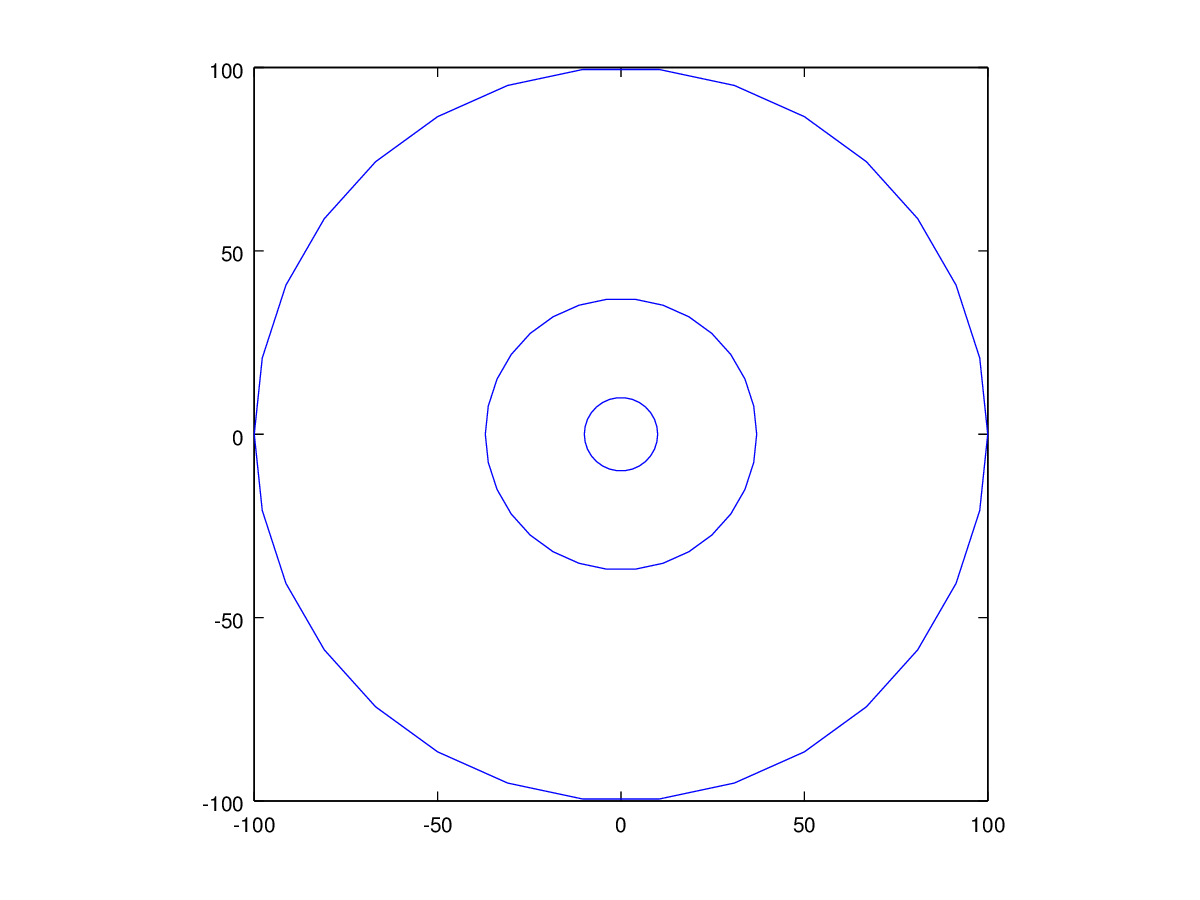
\includegraphics[width=0.49\columnwidth]{../src/experimentos/exp4/iso4A.png}}
\subfigure [4b - 100 radios] {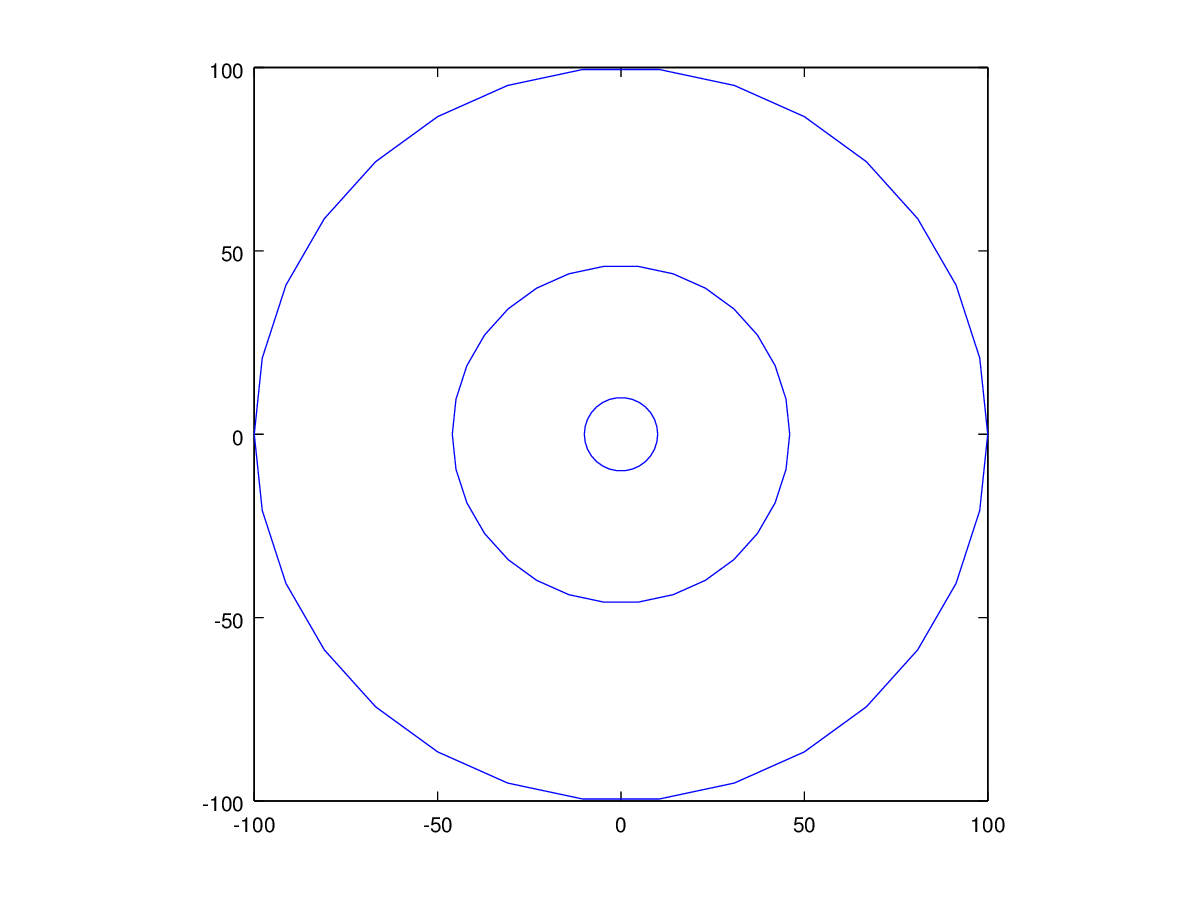
\includegraphics[width=0.49\columnwidth]{../src/experimentos/exp4/iso4b.png}}
\caption{Experimento 4, gráfico de isoterma}
\end{center}
\end{figure}

\par Como se ve en los gráficos, se observa mayor precisión al aumentar la granularidad. La isoterma en el caso que toma mayor cantidad de radios se acerca al borde externo, lo que podría indicar que un test de peligrosidad podría llegar a dar un falso negativo si no se toma la cantidad adecuada de radios, provocando una falla grave en el sistema.

\subsubsection{Experimento 5}

\par Análogamente, en este experimento se observará como varían las temperaturas y la isoterma al modificar la cantidad de ángulos de entrada, manteniendo las demás variables constantes.

\FloatBarrier

\subsubsection{Resultados del experimento 5}

\begin{figure}[ht]
\begin{center}
\subfigure [5a - 10 ángulos] {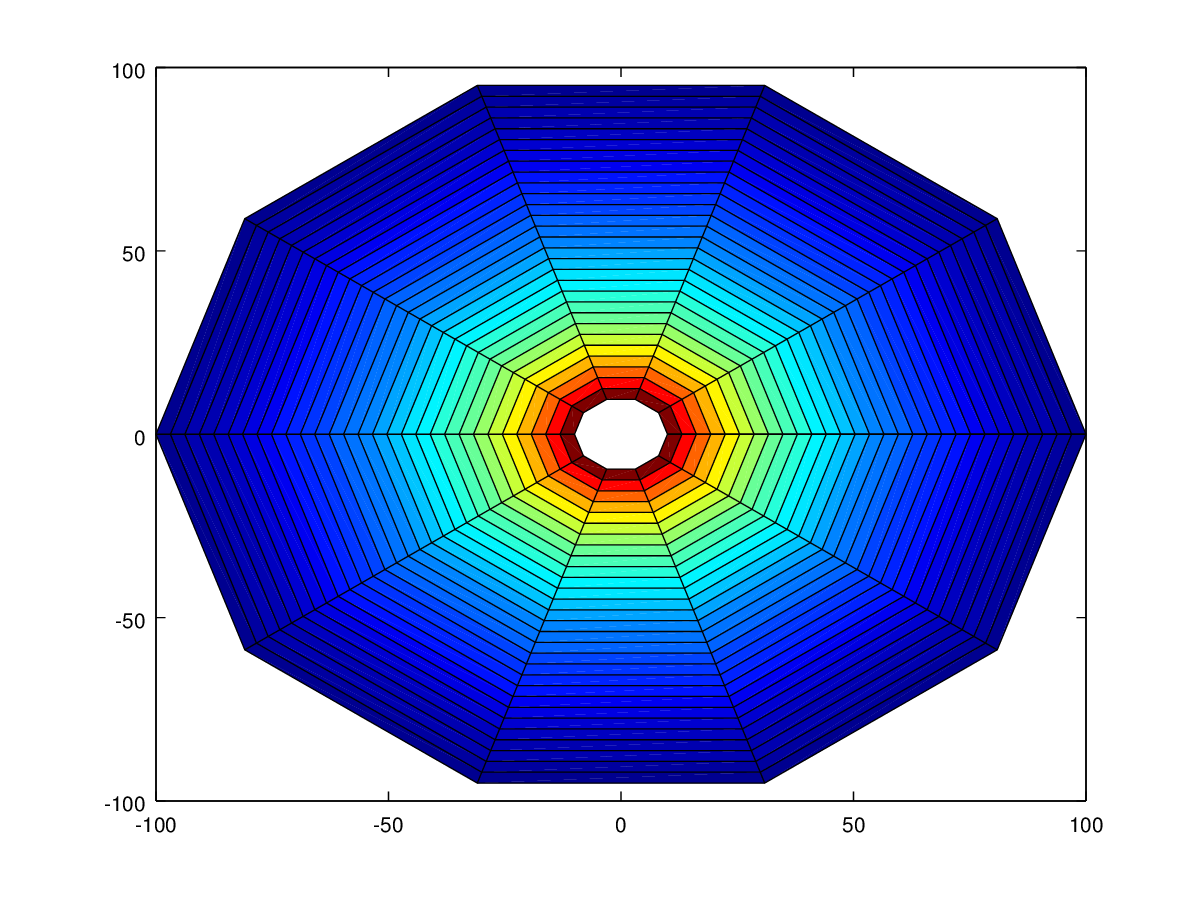
\includegraphics[width=0.49\columnwidth]{../src/experimentos/exp5/calor5a.png}}
\subfigure [5b - 100 ángulos] {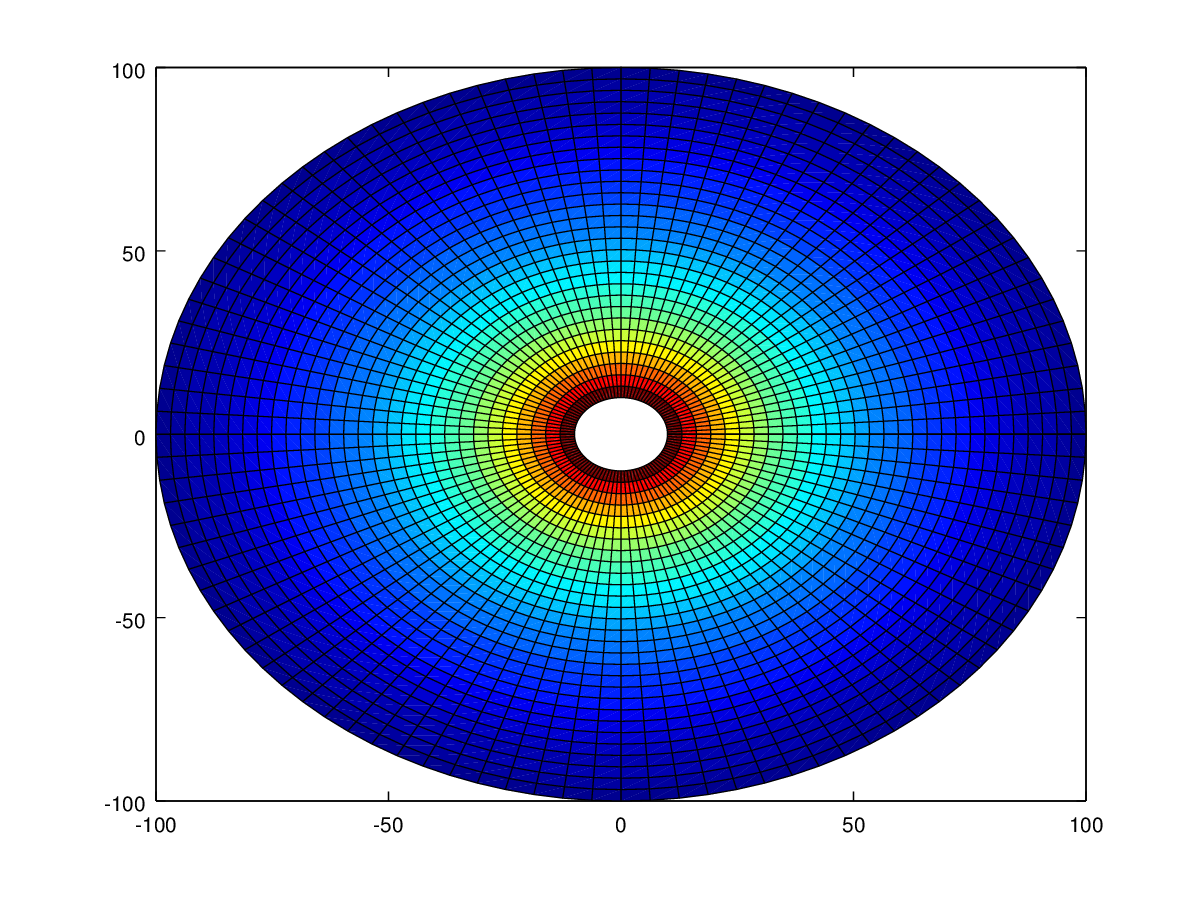
\includegraphics[width=0.49\columnwidth]{../src/experimentos/exp5/calor5b.png}}
\caption{Experimento 5, gráfico de calor}
\end{center}
\end{figure}

\begin{figure}[ht]
\begin{center}
\subfigure [5a - 10 ángulos] {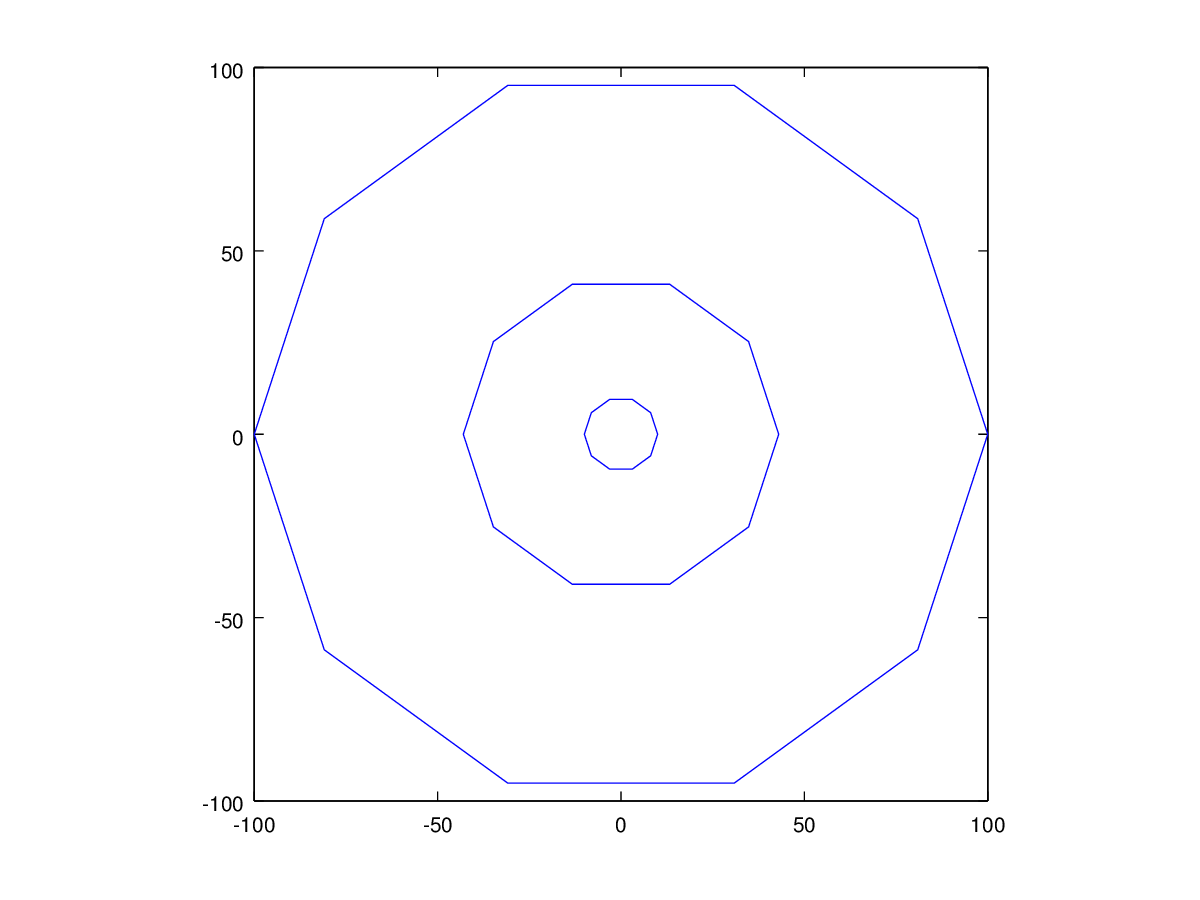
\includegraphics[width=0.49\columnwidth]{../src/experimentos/exp5/iso5a.png}}
\subfigure [5b - 100 ángulos] {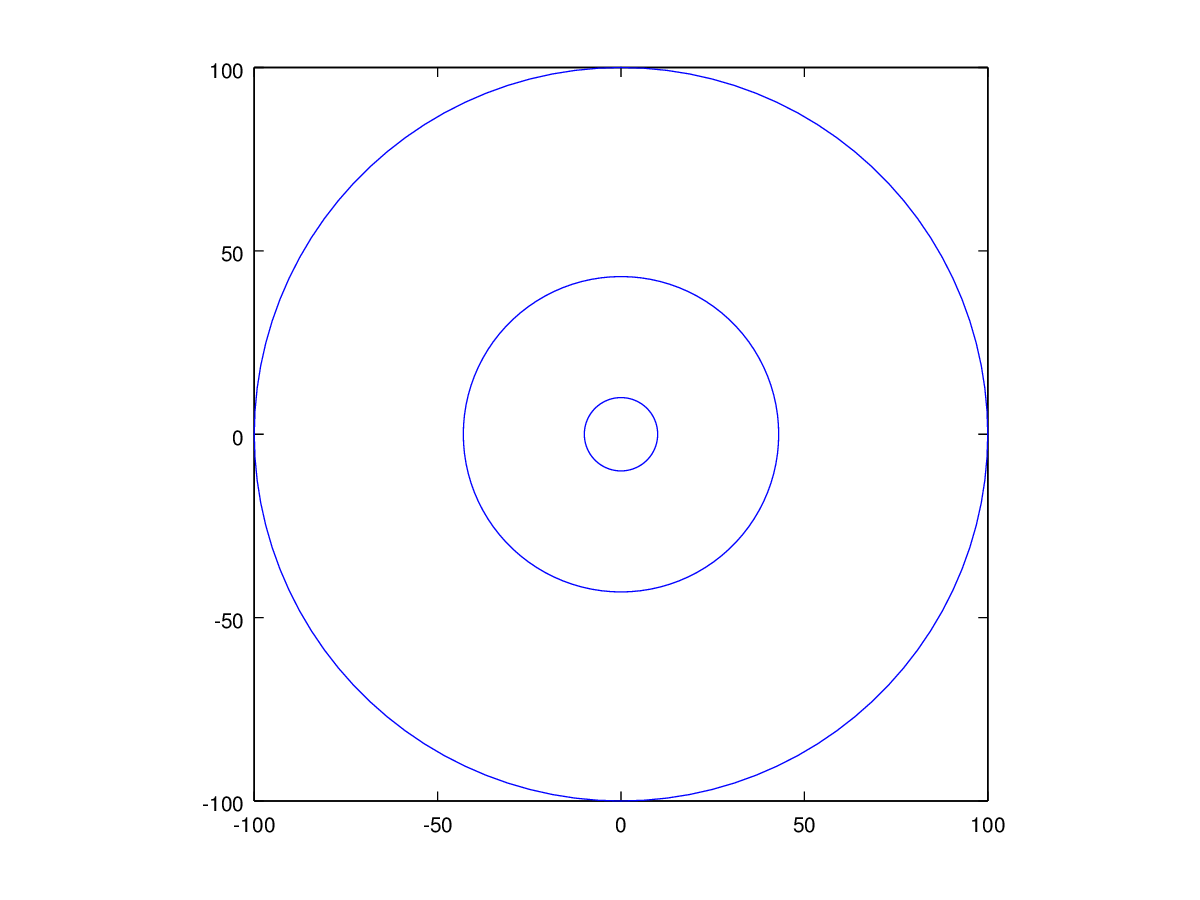
\includegraphics[width=0.49\columnwidth]{../src/experimentos/exp5/iso5b.png}}
\caption{Experimento 5, gráfico de isoterma}
\end{center}
\end{figure}

\par Al igual que en el experimento anterior, la precisión aumenta al aumentar la cantidad de ángulos. En este caso la forma de la isoterma se ve que se asemeja a un círculo al aumentar la granularidad en los ángulos, que es la verdadera forma del horno. Esto es importante ya que decidir si se encuentra en condiciones de peligro con una isoterma tan deformada podría dar resultados incorrectos.

\subsubsection{Experimento 6}

\par Por último, en este experimento se desea comparar los resultados al aumentar la granularidad en ambas variables (radios y ángulos), con el objetivo de determinar cuál de ellas es más importante, refiriéndonos a su granularidad, a la hora de lograr una isoterma que permita calcular la peligrosidad de manera correcta.


\subsubsection{Resultados del experimento 6}

\begin{figure}[ht]
\begin{center}
\subfigure [6a - 10 radios y 10 ángulos] {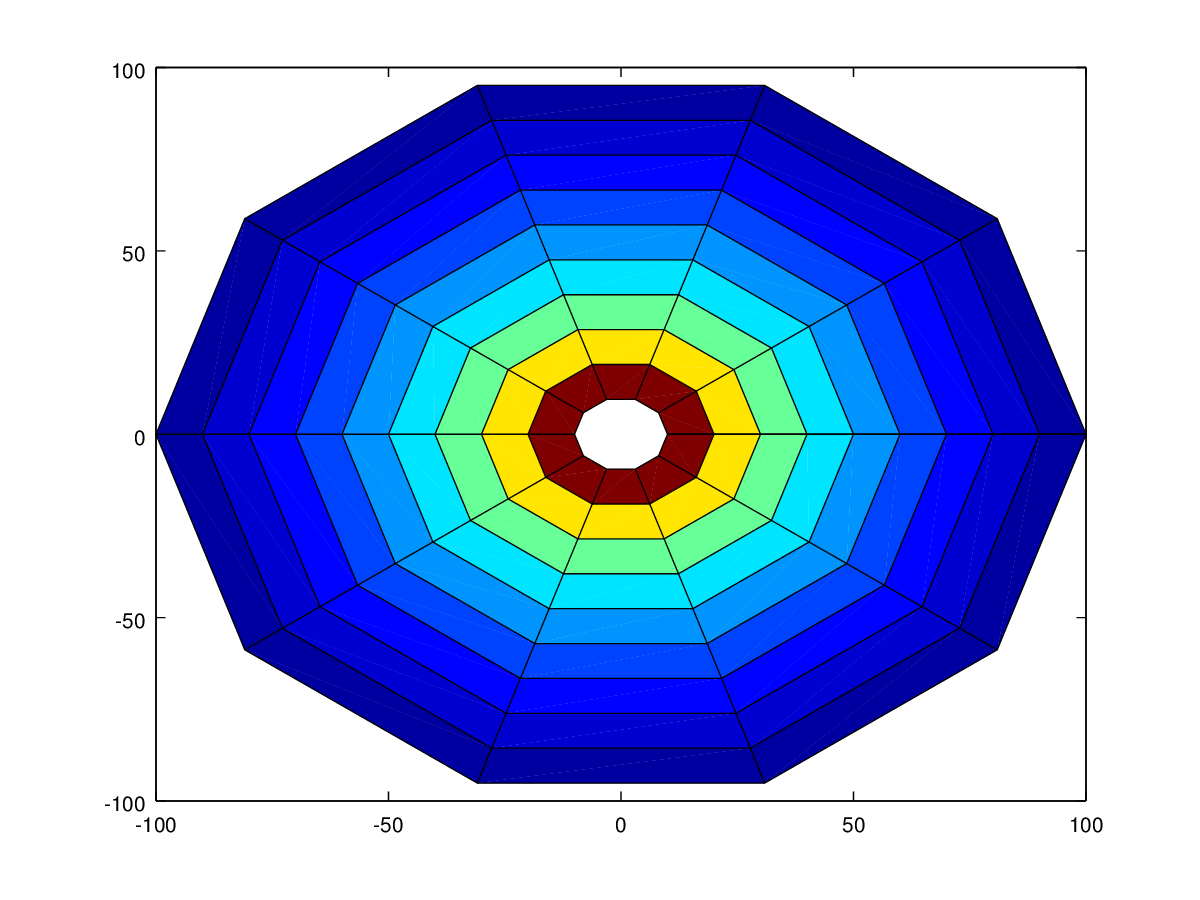
\includegraphics[width=0.49\columnwidth]{../src/experimentos/exp6/calor6a.png}}
\subfigure [6b - 100 radios y 100 ángulos] {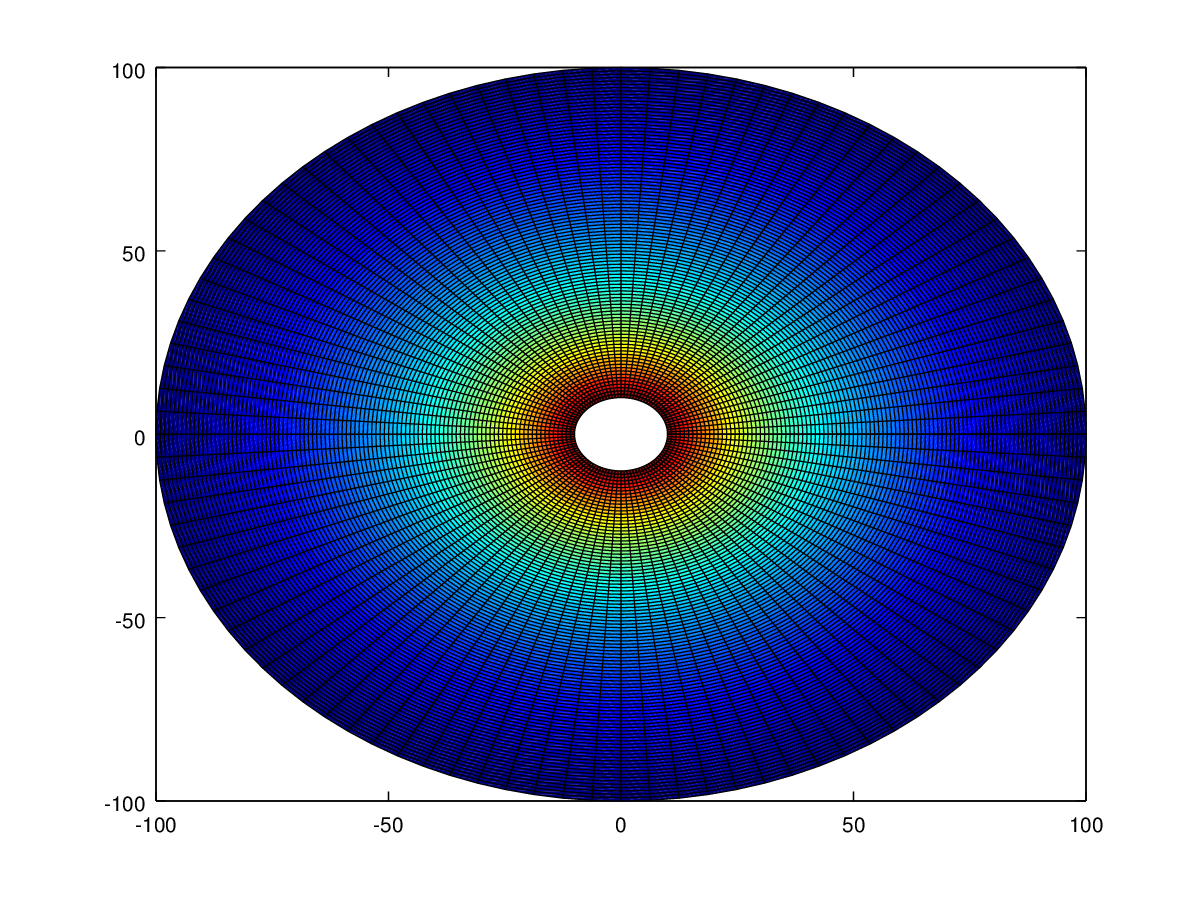
\includegraphics[width=0.49\columnwidth]{../src/experimentos/exp6/calor6b.png}}
\caption{Experimento 6, gráfico de calor}
\end{center}
\end{figure}

\begin{figure}[ht]
\begin{center}
\subfigure [6a - 10 radios y 10 ángulos] {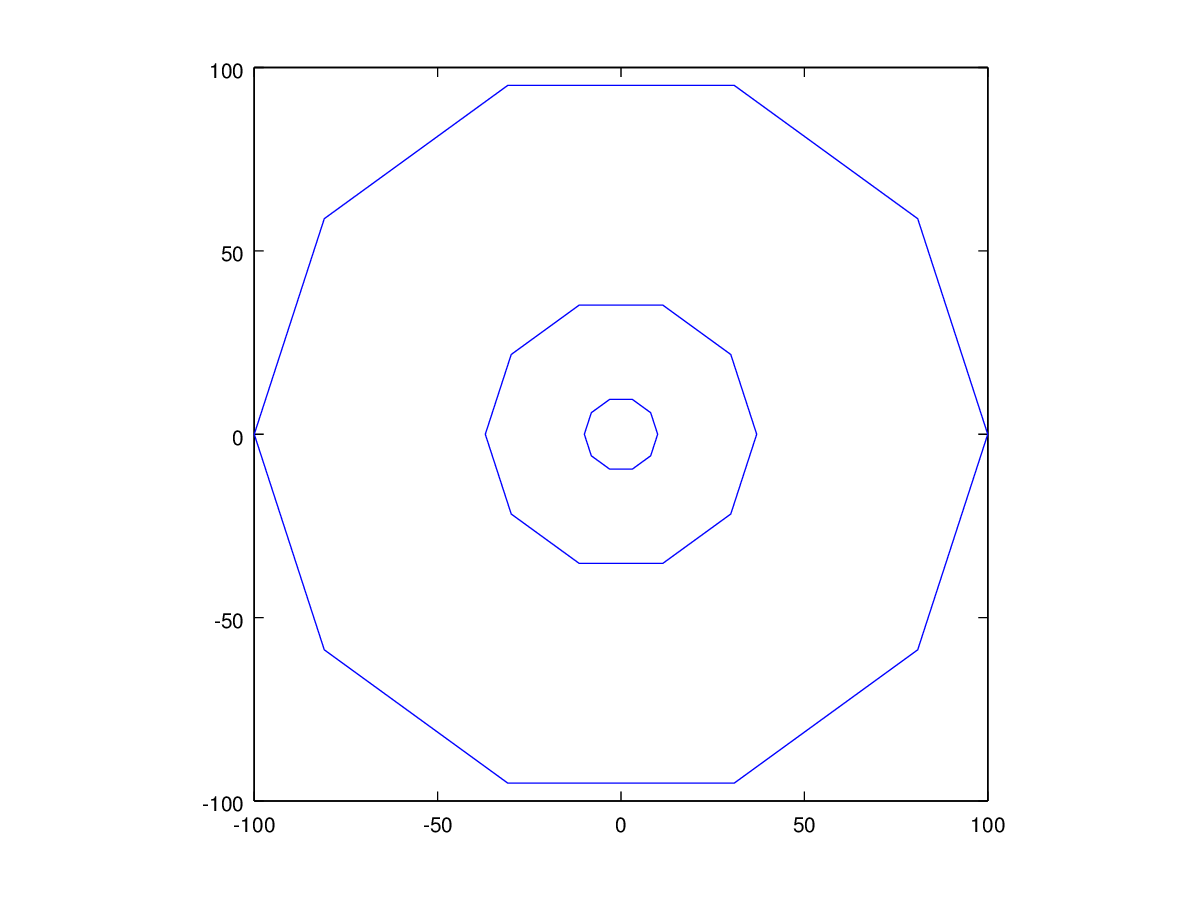
\includegraphics[width=0.49\columnwidth]{../src/experimentos/exp6/iso6a.png}}
\subfigure [6b - 100 radios y 100 ángulos] {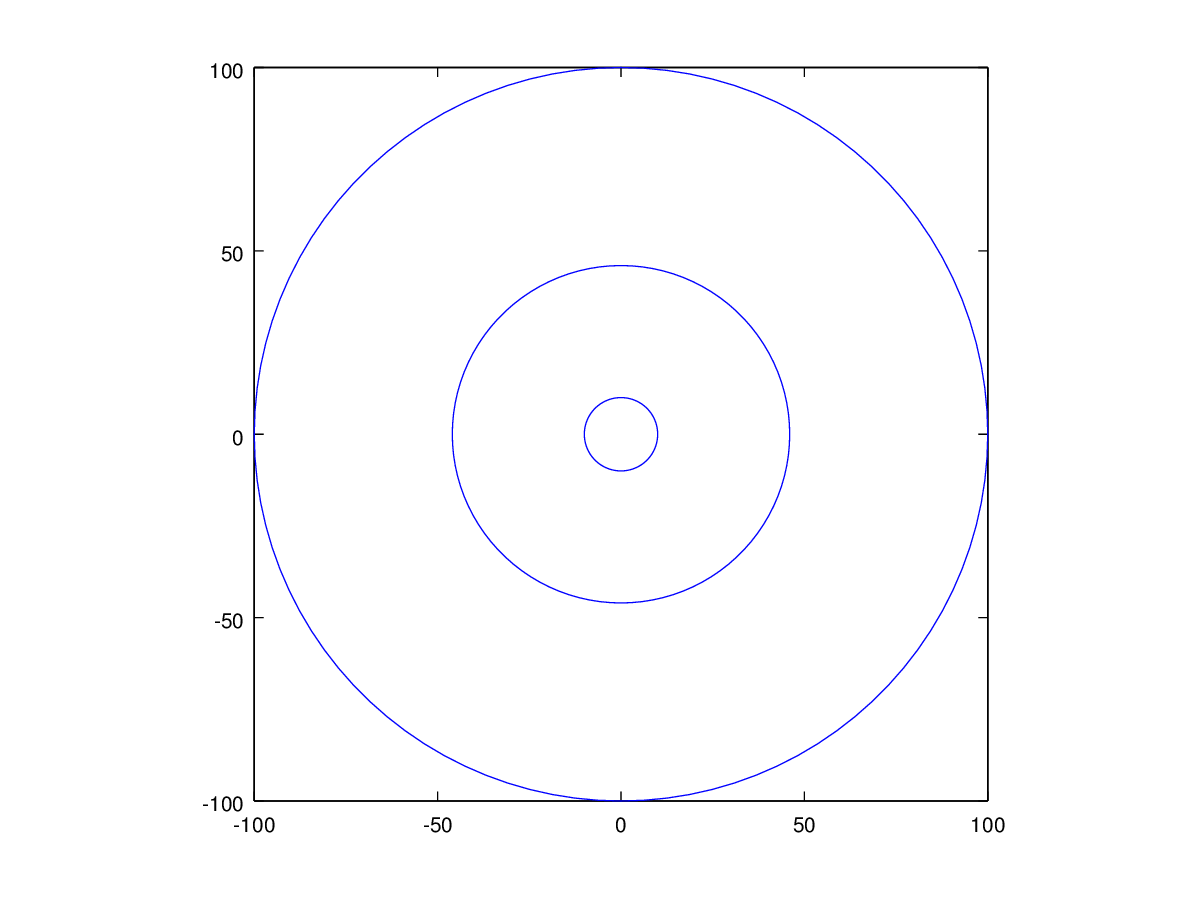
\includegraphics[width=0.49\columnwidth]{../src/experimentos/exp6/iso6b.png}}
\caption{Experimento 6, gráfico de isoterma}
\end{center}
\end{figure}

\par Concluimos que la granularidad es una variable muy importante a la hora de determinar las temperaturas del horno, más allá de que aumente la complejidad temporal del algoritmo. Como se pudo ver en estos experimentos, disminuir la granularidad de alguna de las variables puede producir resultados incorrectos a la hora de calcular peligrosidad. Además, vemos que ambas variables (radios y ángulos) tienen igual importancia, a pesar de que el gráfico para poca cantidad de ángulos se vea más deformado a simple vista.

\subsubsection{Experimento 7}
\par Contamos con distintas formas de calcular la isoterma:
\begin{itemize}
\item Redondear al punto mas cercano.
\item Promediar el punto entre los mas cercanos.
\end{itemize}

\par Creemos que cuanto mayor distancia entre puntos de discretización, mayor va a ser la distancia entre el punto calculado por el procedimiento 1 y el verdadero valor de radio de la isoterma. En cambio con el procedimiento 2 nos aseguramos acercarnos 'un poco mas' (mas allá de la distancia entre radios).

\subsubsection{Primera entrada para el experimento 7}
\par Para simular este caso particular vamos a tomar un estado donde el radio interno es 10mts y el externo es 10000mts. Tomamos tan solo 30 radios, por lo que la distancia entre radios es de 333mts. Tomamos temperaturas internas alternantes entre 5500, 1000 y 550 para lograr una isoterma no circular y variable. Planteamos como hipótesis que en el caso del procedimiento 1 la isoterma va a ser poco variable, y que, en caso de verse un salto, va a ser brusco (de 333mts) entre cada punto. Mientras que con el procedimiento 2 van a poder notarse mas cambios, pero mas leves, ya que al ir promediando va a variar entre puntos intermedios (menores a 333mts).

\subsubsection{Resultados para la primera entrada para el experimento 7}

\begin{figure}[ht]
\begin{center}
\subfigure [Procedimiento 1] {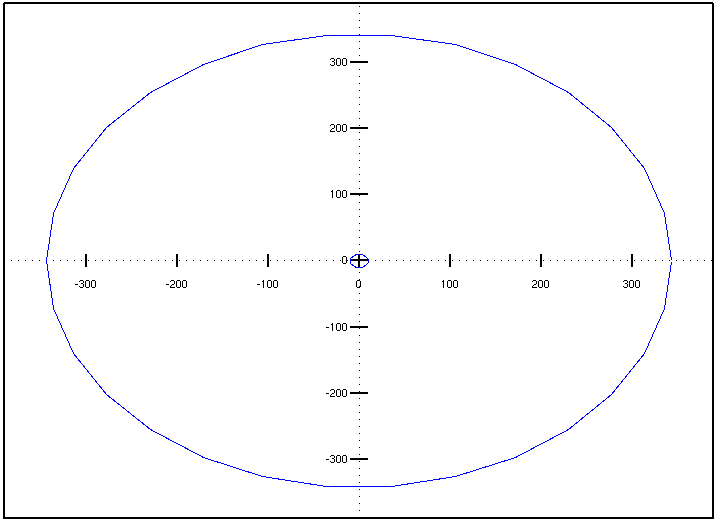
\includegraphics[width=0.49\columnwidth]{../src/experimentos/exp7/se_pudrio_todo/1/isoterma.png}}
\subfigure [Procedimiento 2] {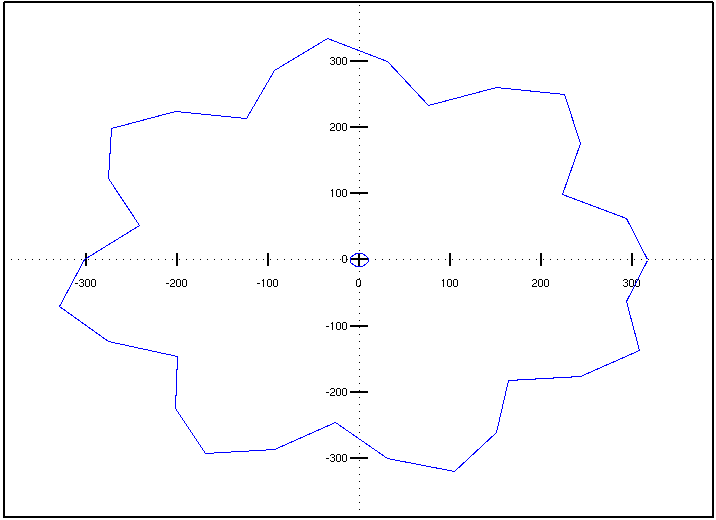
\includegraphics[width=0.49\columnwidth]{../src/experimentos/exp7/promedio/1/isoterma.png}}
\caption{Experimento 7, primera entrada}
\end{center}
\end{figure}

\par En los gráficos se puede notar la diferencia entre los resultados del procedimiento 1 y el 2. En el caso del 1, al mantenerse la isoterma cerca del radio 343mts se redondea tomando el punto 343mts. Esto se da en todos los ángulos, por lo que se obtiene una isoterma circular. Mientras que en el caso del procedimiento 2 se pueden distinguir los cambios y variaciones de la isoterma acercándose por valores intermedios de los radios, consiguiéndose así saltos leves.

\subsubsection{Segunda entrada para el Experimento 7}
\par Vamos a modificar la entrada dejando solo temperaturas externas variables entre 1500 y 1200. Creemos que esto no va a modificar el gráfico de la isoterma según el procedimiento 1, ya que si disminuimos la diferencia de las temperaturas las isotermas de los diferentes ángulos deberían ocupar radios mas cercanos entre sí. Si creemos que va a cambiar el gráfico de la isoterma del procedimiento 2, ya que si hay poca diferencia entre las temperaturas externas debería acercarse un círculo.

\subsubsection{Resultados para la segunda entrada para el Experimento 7}

\begin{figure}[ht]
\begin{center}
\subfigure [Procedimiento 1] {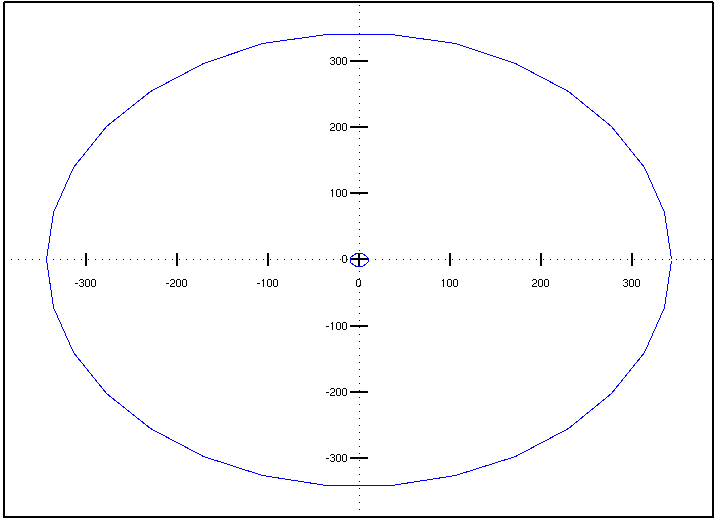
\includegraphics[width=0.49\columnwidth]{../src/experimentos/exp7/se_pudrio_todo/2/isoterma.png}}
\subfigure [Procedimiento 2] {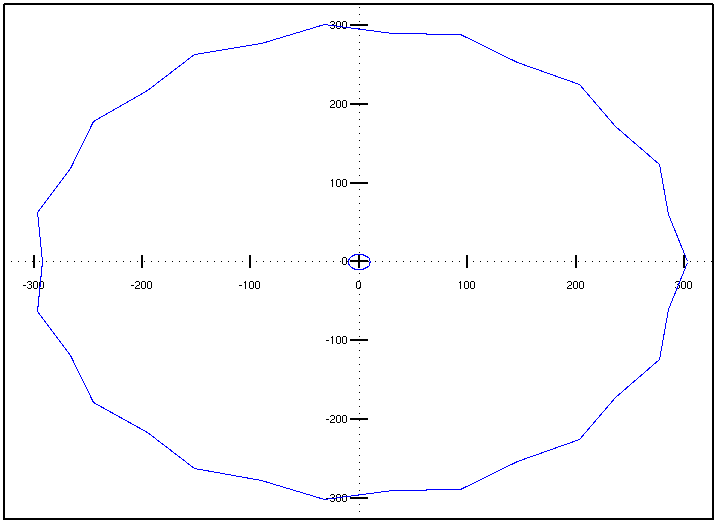
\includegraphics[width=0.49\columnwidth]{../src/experimentos/exp7/promedio/2/isoterma.png}}
\caption{Experimento 7, segunda entrada}
\end{center}
\end{figure}

\par En el gráfico del procedimiento 1, podemos notar que la isoterma tiene forma circular (igual que en A), debido a la poca diferencia entre temperaturas externas y que redondeamos su valor. En cambio en el caso del procedimiento 2 notamos una gran diferencia con respecto al gráfico del A. Como pudimos predecir, al acercar las temperaturas externas entre sí los puntos de la isoterma se posicionan mas cerca y ya no veos saltos tan bruscos. Lo que si podemos ver es que los valores de la isoterma varían entre 2 puntos (al igual que las temperaturas externas).

\subsubsection{Experimento 8}
\par Creemos que podríamos ahorrar tiempo si ejecutamos un estado con pocos radios y usando el procedimiento 2 para calcular la isoterma en vez de usar el procedimiento 1 con mas granularidad de radios. Para esto tomamos un estado con temperaturas externas variables entre 1500 y 1000 grados y vamos a calcular su isoterma 300 utilizando el procedimiento 2 con 10 radios. También calcularemos la misma isoterma utilizando el procedimiento 1 con 20 y 100 radios y compararemos los resultados para ver si podemos aproximar la isoterma utilizando el procedimiento 2 con poca granularidad de radios.

\subsubsection{Resultados del Experimento 8}

\begin{figure}[ht]
\begin{center}
\subfigure [Procedimiento 2 con 10 radios] {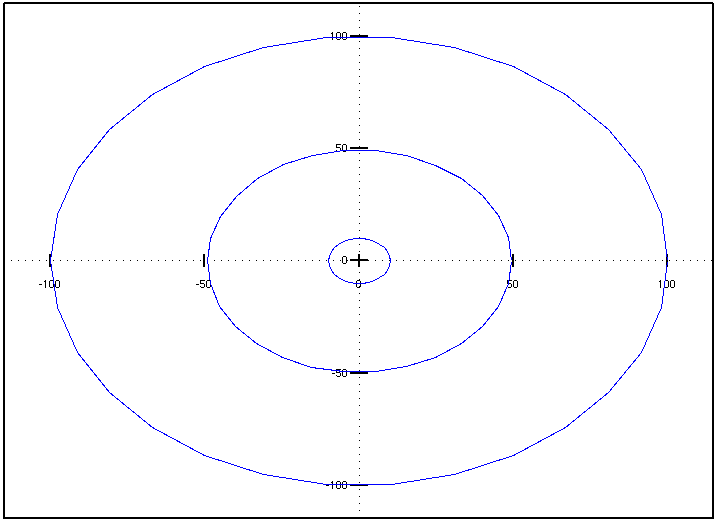
\includegraphics[width=0.49\columnwidth]{../src/experimentos/exp8/promedio/10/isoterma.png}}
\subfigure [Procedimiento 1 con 100 radios] {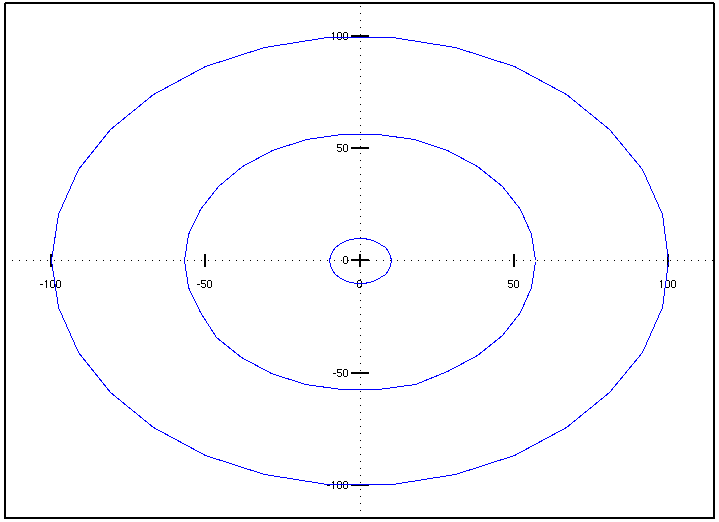
\includegraphics[width=0.49\columnwidth]{../src/experimentos/exp8/gran_spt/100/isoterma.png}}
\caption{Experimento 8}
\end{center}
\end{figure}

\par Como vemos en los gráficos, la isoterma obtenida con el procedimiento 2 nos sirven para aproximar (a grandes rasgos) la posición de la isoterma, pero tomando en cuenta que calcular la isoterma con el procedimiento 1 y 100 radios no nos llevó un tiempo relevante podemos calcularla de esta forma y aproximar mucho mejor la isoterma (sin necesidad de mucho mas tiempo). Así concluimos que nuestro primer pensamiento de que se podía aproximar la isoterma con rapidéz utilizando el procedimiento 2 era correcta, pero solo a grandes rasgos. Y teniendo en cuenta lo dicho antes podemos utilizar el procedimiento 1 sin necesidad de pagar con gran tiempo de ejecución.


\subsection{Resultados con respecto a la Peligrosidad}

\subsubsection{Experimento 9}

\par En este experimento se buscará comparar dos métodos implementados para decidir la peligrosidad de un horno a partir de la isoterma 500.
\par El primero, tan solo se fija si alguno de los puntos de la isoterma 500 sobrepasa una distancia predeterminada al radio externo:

\lstset{language=C++, breaklines=true, basicstyle=\footnotesize}
\begin{lstlisting}[frame=single]
bool estaEnPeligro (vector<double>& isoVec, int ri, int re, double indiceDePeligro)
{
    double sePudrioTodo = ((double) re - ri) * indiceDePeligro;
    for (int i = 0; i < isoVec.size(); i++)
    {
        if (isoVec [i] >= sePudrioTodo) return true;
    }
    return false;
}
\end{lstlisting}

\par El segundo algoritmo, en cambio, calcula la cantidad de puntos en peligro y la compara con la cantidad total de puntos en la circunsferencia, calificándolo como en peligro si éste supera el 40\%. Seleccionamos uno de los casos bordes para mostrar la diferencia entre los métodos, donde la mitad izquierda del horno es más fría (quizás por algún mecanismo de ventilación o enfriamiento) que la de la derecha.

%\lstset{language=C++, breaklines=true, basicstyle=\footnotesize}
%\begin{lstlisting}[frame=single]
%bool estaEnPeligroPromedio (vector<double>& isoVec, int ri, int re, double indiceDePeligro)
%{
%    double sePudrioTodo = ((double) re - ri) * indiceDePeligro;
%    int peligrosos = 0;
%    for (int i = 0; i < isoVec.size(); i++)
%    {
%        if (isoVec [i] >= sePudrioTodo) peligrosos++;
%    }
%    if (peligrosos/isoVec.size() >= 0.4 ){
%        return true;
%    }else{
%        return false;
%    }
%}
%\end{lstlisting}

\subsubsection{Resultados del experimento 9}

\begin{figure}[ht]
\begin{center}
\subfigure [] {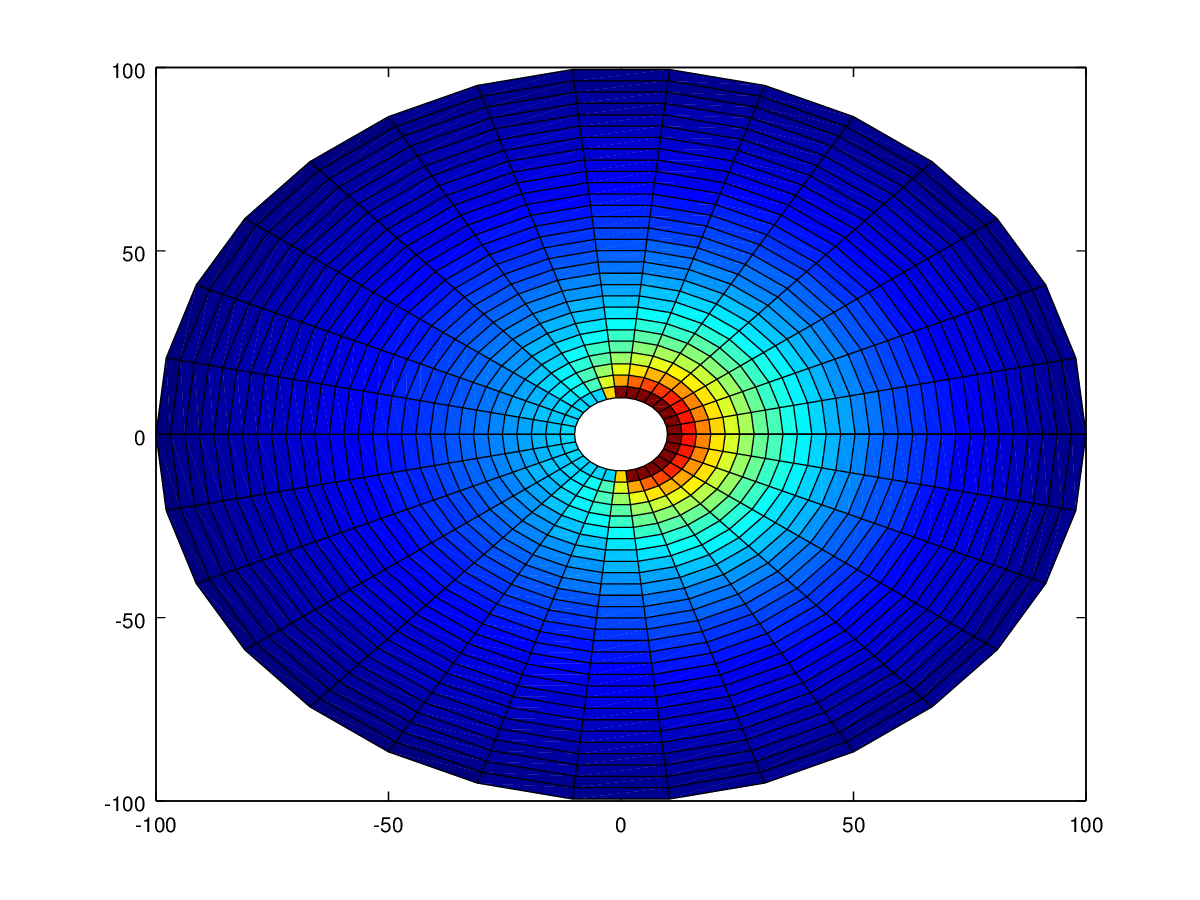
\includegraphics[width=0.5\columnwidth]{../src/experimentos/exp9/promedio/calor01.png}}
\subfigure [] {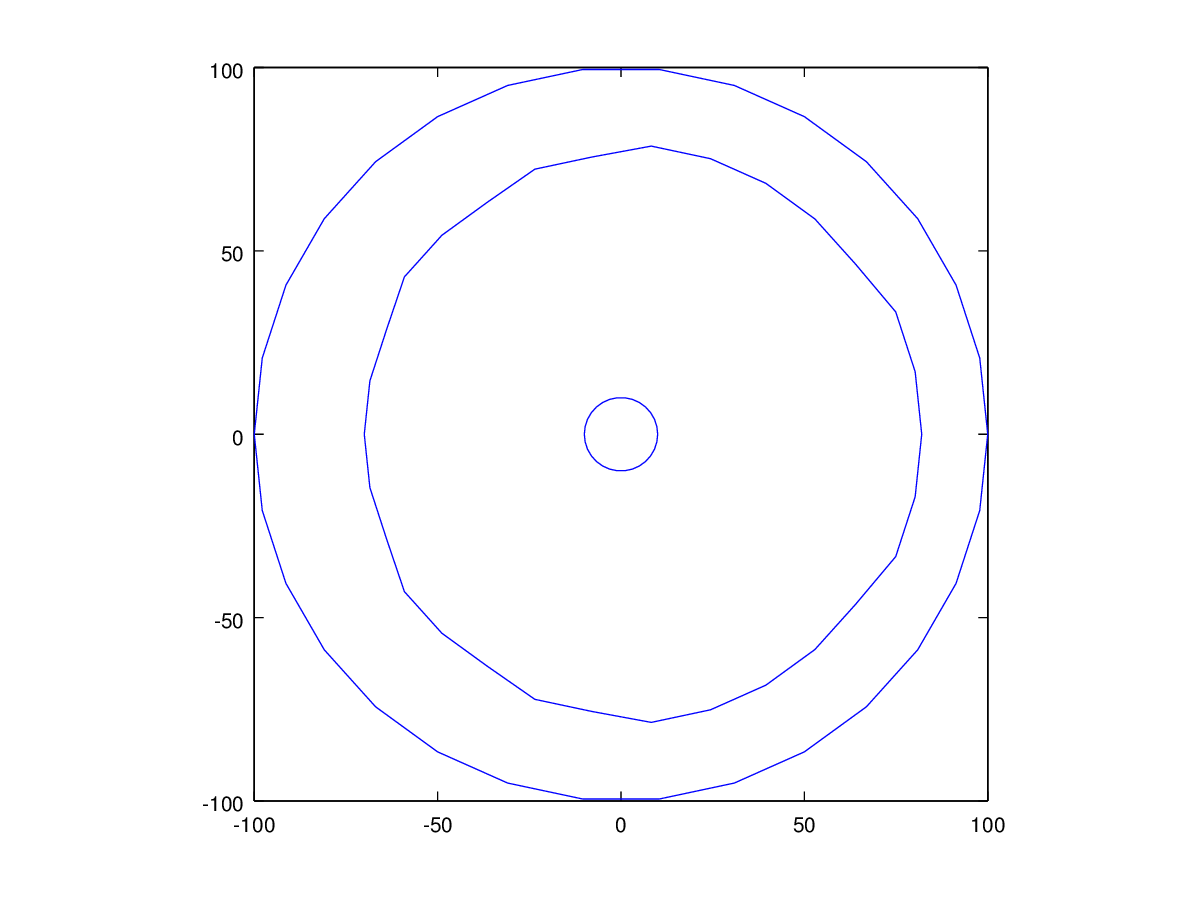
\includegraphics[width=0.49\columnwidth]{../src/experimentos/exp9/promedio/iso01.png}}
\caption{Experimento 9}
\end{center}
\end{figure}

\par estaEnPeligro da PELIGRO
\par estaEnPeligroPromedio da No esta en peligro

\par Para casos bordes como el mostrado en la figura 15, donde el horno tiene temperaturas más frías en un sector que en otro, los resultados de los métodos difieren. Quedará por decidir cuál de los dos es el más convieniente para cada situación: el primero, si nos encontramos en una situación crítica donde el menor exceso de temperatura pueda significar un grave problema; o el segundo, cuando la situación pueda ser más controlable si sólo una parte del horno haya excedido el límite de cercanía al borde externo.




 
\newpage

\section{Conclusiones}

\par En primer lugar, concluimos (como se esperaba), que la Eliminaci\'on Gaussiana optimizada para banda es el algoritmo m\'as eficiente para resolver sistemas con pocos t\'erminos independientes distintos. Gauss result\'o ser m\'as eficiente que LU, pero por un factor muy peque\~no.
\par LU result\'o ser a\'un m\'as eficiente que Gauss optimizada para sistemas con muchos t\'erminos independientes distintos, a pesar de que ambos tienen complejidad cuadr\'atica (en el tama\~no de la matriz) despu\'es de la primera soluci\'on (en el caso de LU, la descomposici\'on original es c\'ubica).
\par La conclusi\'on m\'as interesante que obtuvimos fue respecto al efecto de las optimizaciones de banda: incluso las optimizaciones que originalmente consideramos menores para banda en Gauss y LU tienen un efecto muy significativo en el tiempo de ejecuci\'on de los algoritmos.
\par De estos comentarios se desprende la idea de que contar con cada detalle del sistema a modelar puede permitirnos plantear de mejor manera el problema y la forma en la que lo vamos a resolver, optimizando los resultados que luego se van a obtener. Por ejemplo plantear el sistema de ecuaciones de cierta forma nos permite aprovechar las características de una matriz banda y poder mejorar el rendimiento de nuestro programa.
\par También pudimos acercarnos mas a la investigación, sus formas y métodos, así como la idea de recibir colaboración por parte de especialistas para plantear las formas de resolver el problema, las ecuaciones y datos extras que pueden ayudarnos para dar con la solución y optimizar el proceso.
 
\newpage

\section{Ap\'endices}

\subsection{Apéndice A}

{\bf Enunciado}

Se debe implementar un programa en \verb+C+ o \verb-C++- que tome como entrada los par\'ametros del problema ($r_i$, $r_e$, $m+1$,
$n$, valor de la isoterma buscada, $T_i$, $T_e(\theta)$) que calcule la temperatura dentro de la pared del horno utilizando el
modelo propuesto en la secci\'on anterior y que encuentre la isoterma buscada en funci\'on del resultado obtenido del
sistema de ecuaciones. El m\'etodo para determinar la posici\'on de la isoterma queda a libre elecci\'on de cada grupo y
debe ser explicado en detalle en el informe.

El programa debe formular el sistema obtenido a partir de las ecuaciones (1) - (6) y considerar dos m\'etodos posibles
para su resoluci\'on: mediante el algoritmo cl\'asico de Eliminaci\'on Gaussiana y la Factorizaci\'on LU. Finalmente, el
programa escribir\'a en un archivo la soluci\'on obtenida con el formato especificado en la siguiente secci\'on.

Como ya se ha visto en la materia, no es posible aplicar los m\'etodos propuestos para la resoluci\'on a cualquier
sistema de ecuaciones. Sin embargo, la matriz del sistema considerado en el presente trabajo cumple con ser diagonal dominante (no
estricto) y que, ordenando las variables y ecuaciones convenientemente, es posible armar un sistema de ecuaciones cuya matriz
posee la propiedad de ser \emph{banda}. Luego, se pide demostrar (o al menos dar un esquema de la demostraci\'on)
el siguiente resultado e incluirlo en el informe:

\begin{proposition}
Sea $A \in \mathbb{R}^{n \times n}$ la matriz obtenida para el sistema definido por (1)-(6). Demostrar que es posible
aplicar Eliminaci\'on Gaussiana sin pivoteo.\footnote{Sugerencia: Notar que la matriz es diagonal dominante (no
estrictamente) y analizar qué sucede al aplicar un paso de Eliminaci\'on Gaussiana con los elementos de una fila.} 
\end{proposition}

La soluci\'on del sistema de ecuaciones permitir\'a saber la temperatura en los puntos de la discretizaci\'on. Sin embargo,
nuestro inter\'es es calcular la isoterma 500, para poder determinar si la estructura se encuentra en peligro. Luego, se pide lo siguiente:
\begin{itemize}
\item Dada la soluci\'on del sistema de ecuaciones, proponer una forma de estimar en cada \'angulo de la discretizaci\'on la posici\'on de la 
isoterma 500.
\item En funci\'on de la aproximaci\'on de la isoterma, proponer una forma (o medida) a utilizar para evaluar la peligrosidad de la estructura
en funci\'on de la distancia a la pared externa del horno.
\end{itemize}


En funci\'on de la experimentaci\'on, se busca realizar dos estudios complementarios: por un lado, analizar c\'omo se comporta el sistema y, por otro, 
cu\'ales son los requerimientos computacionales de los m\'etodos. Se pide como m\'inimo realizar los siguientes experimentos:
\begin{enumerate}
\item Comportamiento del sistema.
\begin{itemize}
\item Considerar al menos dos instancias de prueba, generando distintas discretizaciones para cada una de ellas y
comparando la ubicaci\'on de la isoterma buscada respecto de la pared externa del horno. Se sugiere presentar gr\'aficos
de temperatura o curvas de nivel para los mismos, ya sea utilizando las herramientas provistas por la c\'atedra o
implementando sus propias herramientas de graficaci\'on. 
\item Estudiar la proximidad de la isoterma buscada respecto de la pared exterior del horno en funci\'on de distintas 
granularidades de discretizaci\'on y las condiciones de borde. 
\end{itemize}
\item Evaluaci\'on de los m\'etodos.
\begin{itemize}
\item Analizar el tiempo de c\'omputo requerido para obtener la soluci\'on del sistema en funci\'on de la granularidad de 
la discretizaci\'on. Se sugiere presentar los resultados mediante gr\'aficos de tiempo de c\'omputo en funci\'on de alguna 
de las variables del problema.
\item Considerar un escenario similar al propuesto en el experimento 1. pero donde las condiciones de borde (i.e., $T_i$ y $T_e(\theta)$)
cambian en distintos instantes de tiempo. En este caso, buscamos obtener la secuencia de estados de la temperatura en
la pared del horno, y la respectiva ubicaci\'on de la isoterma especificada. Para ello, se considera una secuencia de $ninst$
vectores con las condiciones de borde, y las temperaturas en cada estado es la soluci\'on del correspondiente sistema de
ecuaciones. Se pide formular al menos un experimento de este tipo, aplicar los m\'etodos de resoluci\'on propuestos de
forma conveniente y compararlos en t\'erminos de tiempo total de c\'omputo requerido para distintos valores de $ninst$.
\end{itemize}
\end{enumerate}

De manera opcional, aquellos grupos que quieran ir un poco m\'as all\'a pueden considerar trabajar y desarrollar alguno(s) 
de los siguientes puntos extra:
\begin{enumerate}
\item Notar que el sistema resultante tiene estructura \emph{banda}. Proponer una estructura para aprovechar este hecho en t\'erminos de la
\emph{complejidad espacial} y como se adaptar\'ian los algoritmos de Eliminaci\'on Gaussiana y Factorizaci\'on LU para reducir la
cantidad de operaciones a realizar.
\item Implementar dicha estructura y las adaptaciones necesarias para el algoritmo de Eliminaci\'on Gaussiana.
\item Implementar dicha estructura y las adaptaciones necesarias para el algoritmo de Factorizaci\'on LU. 
\end{enumerate}

Finalmente, se deber\'a presentar un informe que incluya una descripci\'on detallada de los m\'etodos implementados y
las decisiones tomadas, el m\'etodo propuesto para el c\'alculo de la isoterma buscada y los experimentos realizados,
junto con el correspondiente an\'alisis y siguiendo las pautas definidas en el archivo \verb+pautas.pdf+.


\subsection{Apéndice B}

\textbf{Código fuente para la creación de la matriz}
\textbf{}

\lstset{language=C++, breaklines=true, basicstyle=\footnotesize}
\begin{lstlisting}[frame=single]
vector< vector<double> > crearMatriz (double n, double m, double ri, double deltaR, double deltaA){

	vector< vector<double> > matriz((m+1)*n, vector<double>((m+1)*n)); 

	//Completo primeras n filas y ultimas n filas con 1s en la diagonal
	for (int i = 0; i < n; i++){
		matriz[i][i] = 1;
	}
	for (int i = (n*(m+1) - n); i < n*(m+1); i++){
		matriz[i][i] = 1;
	}

	//Completo resto de las ecuaciones usando las formulas
	for (int j = 1; j < m; j++){
		double r = ri + j * deltaR;
		for (int k = 0; k < n; k++){
			//uso para calcular en la matriz la posicion j,k = n x j + k

			// t j,k
			matriz[n*j + k][n*j + k] = (-2*pow(r,2)*pow(deltaA, 2) + r*deltaR*pow(deltaA, 2) - 2*pow(deltaR, 2))/(pow(deltaR, 2)*pow(r, 2)*pow(deltaA, 2));
			
			// t j-1, k
			matriz[n*j + k][n*(j-1) + k] = (r - deltaR)/(pow(deltaR, 2)* r);

			// t j+1, k
			matriz[n*j + k][n*(j+1) + k] = 1 / pow(deltaR, 2);

			// t j, k-1
			matriz[n*j + k][n*j + (k - 1 > 0? k - 1 : n - 1)] = 1 / (pow(r, 2)*pow(deltaA, 2));

			//t j, k+1
			matriz[n*j + k][n*j + (k + 1 < n - 1? k + 1 : 0)] = 1 / (pow(r, 2)*pow(deltaA, 2));
		}
	}
	return matriz;
}
\end{lstlisting}

\textbf{}
\textbf{Código fuente para Eliminación Gaussiana con aprovechamiento de banda}
\textbf{}

\lstset{language=C++, breaklines=true, basicstyle=\footnotesize}
\begin{lstlisting}[frame=single]
void EliminacionParaBanda (vector<vector<double>>& mat, int bandaAltura, int bandaAncho, vector<double>& adjunta)
{
    int h = mat.size();
    int w = mat[0].size();
    for (int PivoteDiagonal = 0; PivoteDiagonal < w; PivoteDiagonal++)
    {
        //corre desde la fila de abajo de la diagonal hasta la bandaAltura-iesima de abajo de la diagonal
        //el resto son 0 por la propiedad banda
        for (int FilaActual = PivoteDiagonal + 1; FilaActual < PivoteDiagonal + bandaAltura && FilaActual < h; FilaActual++)
        {
            if ( mat [FilaActual][PivoteDiagonal] != 0)
            {
                double coeficiente = mat [FilaActual][PivoteDiagonal] / mat [PivoteDiagonal][PivoteDiagonal];
                adjunta [FilaActual] -= adjunta[PivoteDiagonal] * coeficiente;
                //corre desde la columna de la diagonal hasta la bandaAncho-iesima de la derecha de la diagonal
                //el resto son 0 por la propiedad banda
                for (int ColumaEnSuma = PivoteDiagonal; ColumaEnSuma < FilaActual + bandaAncho && ColumaEnSuma < w; ColumaEnSuma++)
                {
                    mat [FilaActual][ColumaEnSuma] -= mat [PivoteDiagonal][ColumaEnSuma] * coeficiente;
                }
            }
        }
    }
}
\end{lstlisting}
 
\section{Referencias}

\par \textit{http://en.cppreference.com/w/}

\textbf{}

\par \textit{R. Burden y J.D.Faires, Análisis numérico, International Thomson Editors, 1998}

\end{document}
